%%%%%%%%%%%%%%%%%%%%%%%%%%%%%%%%%%%%%%%%%%%%%%%%%%%%%%%%%%%%%%%%%%%%%%%%%%%%%%%%%%%%%%%%%%%%%%%%%%%%%%%%%%%%%%%%%%%%%%%%%%%%%%
%%% Template para de LaTeX para o evento XIII Congresso Ibero-Americano de Acústica (FIA 2024)
%%% Baseado no modelo da Revista Acústica e Vibrações da Sobrac (https://revista.acustica.org.br)
%%%	Desenvolvido por por Prof. William D'Andrea Fonseca, Dr. Eng. - Engenharia Acústica UFSM
%%% will.fonseca@eac.ufsm.br
%%% Release 02/06/2024
%%%%%%%%%%%%%%%%%%%%%%%%%%%%%%%%%%%%%%%%%%%%%%%%%%%%%%%%%%%%%%%%%%%%%%%%%%%%%%%%%%%%%%%%%%%%%%%%%%%%%%%%%%%%%%%%%%%%%%%%%%%%%%
\documentclass[12pt, a4paper, twoside, onecolumn]{article}
%%%%%%%%%%%%%%%%%%%%%%%%%%%%%%%%%%%%%%%%%%%%%%%%%%%%%%%%%%%%%%%%%%%%%%%%%%%%%%%%%%%%%%%%%%%%%%%%%%%%%%%%%%%%%%%%%%%%
% \usepackage[english,spanish,es-tabla,brazil]{babel} % Para artigo em português
% \usepackage[english,brazil,spanish,es-tabla]{babel} % Para artíclo en español
\usepackage[spanish,es-tabla,brazil,english]{babel} % For article in english

\usepackage{FIA2024} %%% Template basics
%%%%%%%%%%%%%%%%%%%%%%%%%%%%%%%%%%%%%%%%%%%%%%%%%%%%%%%%%%%%%%%%%%%%%%%%%%%%%%%%%%%%%%%%%%%%%%%%%%%%%%%%%%%%%%%%%%%%
%%% Select language options

% For paper in Spanish words uncomment the line below
 % \Resumen

% For paper in English uncomment the line below
\SuppressResumo 
%%%%%%%%%%%%%%%%%%%%%%%%%%%%%%%%%%%%%%%%%%%%%%%%%%%%%%%%%%%%%%%%%%%%%%%%%%%%%%%%%%%%%%%%%%%%%%%%%%%%%%%%%%%%%%%%%%%%
%%%%%%%%%%%%%%%%%%%%%%%%%%%%%%%%%%%%%%%%%%%%%%%%%%%%%%%%%%%%%%%%%%%%%%%%%%%%%%%%%%%%%%%%%%%%%%%%%%%%%%%%%%%%%%%%%%%%
%%% Dados do artigo

\Authors{Fonseca,~W.~D'A.} % Para metadata do PDF || For PDF metadata

% Use a estrutura "Sobrenome, N." || Utilice la estructura "Apellido, N." || Use the structure "Last name, N."
\AuthorsAffiliations{Fonseca,~W.~D'A.$^1$; Sobrenome, N.$^2$} 
% Use números para afiliações || Utilice números para afiliaciones || Use numbers for affiliations

%% Use apenas UMA linha para autores com a mesma afiliação, declarando apenas diferentes emails
%% Quando houver autores de afiliações diferentes, use uma nova linha

%% Use solo UNA línea para autores con la misma afiliación, declarando solo correos electrónicos diferentes
%% Cuando hay autores con diferentes filiaciones, utilizar una nueva línea

%% Use only ONE line for authors with the same affiliation, declaring only different emails
%% When there are authors with different affiliations, use a new line

\Affiliations{ $^1$\,Acoustical Engineering, Federal University of Santa Maria, Santa Maria, RS, Brazil, will.fonseca@eac.ufsm.br\\[3pt]
						  $^2$\,Acoustical Engineering, FIA University, City, Country, email@email.com\\[-1pt]}

%% Português
\TitleComplete{Instructions and article template for the XIII~Ibero-American Congress of Acoustics (FIA 2024)} % Título completo
\TitleShort{Instructions and article template for the XIII~Ibero-American Congress of Acoustics (FIA 2024)}    % Título curto (se for necessário) para o cabeçalho da página

%% Español
% \TitleComplete{Instrucciones y modelo de artículo para el XIII~Congreso Iberoamericano de Acústica (FIA 2024)}
% \TitleShort{Instrucciones y modelo de artículo para el XIII~Congreso Iberoamericano de Acústica (FIA 2024)}    % Título corto (si es necesario) para el encabezado de la página.


\TitleEnglish{Instructions and article template for the XIII~Ibero-American Congress of Acoustics (FIA 2024)}     % Title in English

\PalavrasChave{artigo técnico, FIA, acústica, vibrações} % Palavras-chave ou/o Palabras clave
\Keywords{technical paper, FIA, acoustics, vibration}    % Keywords

%% Resumen ou/o Resumo 
\Resumo{
%%% Português
% Este documento contém instruções para a escrita de artigos para o XIII Congresso Ibero-Americano de Acústica (FIA 2024). Esse campo é destinado ao resumo do artigo que deve ter entre 150 e 200 palavras. O resumo, palavras-chave, \textit{title}, \textit{abstract} e \textit{keywords} devem ser colocados na primeira página do artigo, buscando não se estender para a segunda página.  O resumo deve fazer uma apresentação concisa do artigo técnico científico, contendo, uma introdução, o objetivo, uma síntese da metodologia, o principal resultado e a principal conclusão (preferencialmente nessa ordem). Não é necessário separar em itens ou seções dentro do resumo. Assim, o leitor pode conhecer a essência do conteúdo do artigo. Lembre-se que o resumo é como o \textit{trailer} de um filme, as pessoas ficarão interessadas em ler completamente o artigo se o resumo lhes interessar. O resumo não deve conter informações novas não contidas no artigo; abreviações indefinidas; discussão prévia de outra literatura; referências e citações e excesso de detalhes acerca dos métodos empregados. Ele também não é o parágrafo de introdução do documento, isso deve ser colocado no início do texto. Utilize apenas informações úteis e relevantes, faça um exercício de empatia com o possível leitor interessado. Para se obter um resumo coeso, elegante e de acordo com o artigo, escreva uma prévia, realize a escrita completa do documento e, ao final, revise-o observando se o conteúdo dele reflete de forma consistente o teor do documento. Seguindo o resumo, o autor deve listar até cinco palavras-chave (evite colocar as mesmas palavras que formam o título do artigo). Após essa etapa, há ainda o título, resumo e palavras-chave em inglês.
%%%%% Español
% Este documento contiene instrucciones para la redacción de artículos para el XIII~Congreso Iberoamericano de Acústica (FIA 2024). Este campo está destinado al resumen del artículo, que debe tener entre 150 y 200 palabras. El resumen, las palabras clave, \textit{title}, \textit{abstract} y \textit{keywords} deben colocarse en la primera página del artículo, procurando no extenderse a la segunda página. El resumen debe hacer una presentación concisa del artículo técnico-científico, conteniendo una introducción, el objetivo, una síntesis de la metodología, el principal resultado y la principal conclusión (preferiblemente en ese orden). No es necesario separar en ítems o secciones dentro del resumen. Así, el lector puede conocer la esencia del contenido del artículo. Recuerde que el resumen es como el \textit{tráiler} de una película; las personas estarán interesadas en leer completamente el artículo si el resumen les interesa. El resumen no debe contener información nueva no incluida en el artículo; abreviaturas indefinidas; discusión previa de otra literatura; referencias y citas ni exceso de detalles sobre los métodos empleados. Tampoco es el párrafo de introducción del documento; esto debe colocarse al inicio del texto. Utilice solo información útil y relevante; haga un ejercicio de empatía con el posible lector interesado. Para obtener un resumen cohesionado, elegante y acorde al artículo, escriba una versión preliminar, realice la redacción completa del documento y, al final, revíselo observando si su contenido refleja de manera consistente el contenido del documento. Siguiendo el resumen, el autor debe listar hasta cinco palabras clave (evite colocar las mismas palabras que forman el título del artículo). Después de esta etapa, aún debe incluir el título, resumen y palabras clave en inglés.
%%%
}

\Abstract{
This document contains instructions for writing papers for the XIII~Ibero-American Congress of Acoustics (FIA 2024).
This field is intended for the abstract of the article, which must contain between 150 and 200 words. The elements \textit{resumo}, \textit{palavras-chave}, title, abstract, and keywords should constitute the first page (i.e., avoid extending them to the second page). The abstract should make a concise presentation of the scientific-technical article, containing an introduction, the objective, a synthesis of the methodology, the main result, and the final conclusion (preferably in that order). Separate items or sections are not required within the abstract. Thus, the reader may acknowledge the essence of the article content. Remember that the abstract is like a movie trailer, people will consider reading the complete article if the abstract is interesting. The abstract should not contain new information not contained within the article; undefined abbreviations; previous discussion of another literature; references and citations; or excessive detail about the methods employed. It is also not the introductory paragraph of the work; this should be placed at the beginning of the text. Use only relevant and useful information, exercising empathy with prospective readers. For a cohesive and elegant abstract that represents the article, write a preview, complete the paper, and then review it by looking at whether its content consistently reflects the content of the document. Following the abstract, the author should list up to five keywords (avoid using the same words contained in the article’s title). After this step, there are also title, abstract, and keywords in English.
}

\Metadata % Includes the metada into the PDF
%%%%%%%%%%%%%%%%%%%%%%%%%%%%%%%%%%%%%%%%%%%%%%%%%%%%%%%%%%%%%%%%%%%%%%%%%%%%%%%%%%%%%%%%%%%%%%%%%%%%%%%%%%%%%%%%%%%%
%%%%%%%%%%%%%%%%%%%%%%%%%%%%%%%%%%%%%%%%%%%%%%%%%%%%%%%%%%%%%%%%%%%%%%%%%%%%%%%%%%%%%%%%%%%%%%%%%%%%%%%%%%%%%%%%%%%%
\begin{document} \setcounter{page}{1} %%%%%%%%%%%%%%%%%%%%%%%%%%%%%%%%%%%%%%%%%%%%%%%%%%%%%%%%%%%%%%%%%%%%%%%%%%%%%%%%%%%%%%%%%%%%%%%%%%%%%%%%%%%%%%%%%%%%
%%% Template para de LaTeX para o evento 12º Congresso Iberoamericano de Acústica 
%%%                      em conjunto com XXIX Encontro da Sobrac
%%% Baseado no modelo da Revista Acústica e Vibrações da Sobrac
%%% Release 19/04/2022
%%%	Desenvolvido por por Prof. William D'Andrea Fonseca, Dr. Eng. - Engenharia Acústica UFSM
%%% will.fonseca@eac.ufsm.br
%%%%%%%%%%%%%%%%%%%%%%%%%%%%%%%%%%%%%%%%%%%%%%%%%%%%%%%%%%%%%%%%%%%%%%%%%%%%%%%%%%%%%%%%%%%%%%%%%%%%%%%%%%%%%%%%%%%%
%%%%%%%%%%%%%%%%%%%%%%%%%%%%%%%%%%%%%%%%%%%%%%%%%%%%%%%%%%%%%%%%%%%%%%%%%%%%%%%%%%%%%%%%%%%%%%%%%%%%%%%%%%%%%%%%%%%%
%% Estilo do artigo
\pagestyle{plain}
%%%%%%%%%%%%%%%%%%%%%%%%%%%%%%%%%%%%%%%%%%%%%%%%%%%%%%%%%%%%%%%%%%%%%%%%%%%%%%%%%%%%%%%%%%%%%%%%%%%%%%%%%%%%%%%%%%%%
%%% Primeira página
\thispagestyle{firststyle}
% \newgeometry{top=2.1cm, bottom=2cm, left=1.9cm, right=1.9cm, headsep=5mm}
%%%%%%%%%%%%%%%%%%%%%%%%%%%%%%%%%%%%%%%%%%%%%%%%%%%%%%%%%%%%%%%%%%%%%%%%%%%%%%%%%%%%%%%%%%%%%%%%%%%%%%%%%%%%%%%%%%%%
\begin{textblock}{200}(150.2,283.51)
\fontsize{8}{8}\selectfont\sffamily 
DOI:~\href{https://doi.org/\DOIArtigo}{\DOIArtigo}
\end{textblock}
%%% Título
\begin{textblock}{170}(37,12)

\includegraphics[width=0.82\textwidth,page=1]{FIA-logo.pdf}
\end{textblock}

\twocolumn[
\begin{@twocolumnfalse}
\vspace{60pt}
\begin{center}
{\fontsize{18}{22}\selectfont\bfseries 
%% Título
%%%%%%%%%%%%%%%%%%%%%%%%%%%%%%%%%%%%%%%%%%%%%%%%%%%%%%%%%%%%%%%%%%%%%%%%%%%%%%%%%%%%%%%%%%%%%%%%%%%%%%%%%%%%%%%%%%%%
\TituloCompletoArtigo \bookmark[page=1,level=1]{Título e Resumo}
%%%%%%%%%%%%%%%%%%%%%%%%%%%%%%%%%%%%%%%%%%%%%%%%%%%%%%%%%%%%%%%%%%%%%%%%%%%%%%%%%%%%%%%%%%%%%%%%%%%%%%%%%%%%%%%%%%%%
\par}

%%%%%%%%%%%%%%%%%%%%%%%%%%%%%%%%%%%%%%%%%%%%%%%%%%%%%%%%%%%%%%%%%%%%%%%%%%%%%%%%%%%%%%%%%%%%%%%%%%%%%%%%%%%%%%%%%%%
%%%%%%%%%%%%%%%%%%%%%%%%%%%%%%%%%%%%%%%%%%%%%%%%%%%%%%%%%%%%%%%%%%%%%%%%%%%%%%%%%%%%%%%%%%%%%%%%%%%%%%%%%%%%%%%%%%%
\vspace{12pt}
{\fontsize{11}{13}\selectfont \bfseries 
%% Autores
%%%%%%%%%%%%%%%%%%%%%%%%%%%%%%%%%%%%%%%%%%%%%%%%%%%%%%%%%%%%%%%%%%%%%%%%%%%%%%%%%%%%%%%%%%%%%%%%%%%%%%%%%%%%%%%%%%%
\AutoresFiliacoesArtigo
%%%%%%%%%%%%%%%%%%%%%%%%%%%%%%%%%%%%%%%%%%%%%%%%%%%%%%%%%%%%%%%%%%%%%%%%%%%%%%%%%%%%%%%%%%%%%%%%%%%%%%%%%%%%%%%%%%%
\par}

\vspace{2mm}
{\fontsize{9}{11}\selectfont 
%% Filiações
%%%%%%%%%%%%%%%%%%%%%%%%%%%%%%%%%%%%%%%%%%%%%%%%%%%%%%%%%%%%%%%%%%%%%%%%%%%%%%%%%%%%%%%%%%%%%%%%%%%%%%%%%%%%%%%%%%%
\FiliacoesArtigo
%%%%%%%%%%%%%%%%%%%%%%%%%%%%%%%%%%%%%%%%%%%%%%%%%%%%%%%%%%%%%%%%%%%%%%%%%%%%%%%%%%%%%%%%%%%%%%%%%%%%%%%%%%%%%%%%%%%%
\par}
\end{center}

\vspace{-5mm}{\color{FIABlue}\rule{\textwidth}{0.4pt}}
%%%%%%%%%%%%%%%%%%%%%%%%%%%%%%%%%%%%%%%%%%%%%%%%%%%%%%%%%%%%%%%%%%%%%%%%%%%%%%%%%%%%%%%%%%%%%%%%%%%%%%%%%%%%%%%%%%%%
%%%%%%%%%%%%%%%%%%%%%%%%%%%%%%%%%%%%%%%%%%%%%%%%%%%%%%%%%%%%%%%%%%%%%%%%%%%%%%%%%%%%%%%%%%%%%%%%%%%%%%%%%%%%%%%%%%%%
%%% Resumo e palavras-chave
\ResumoTexto
%%%%%%%%%%%%%%%%%%%%%%%%%%%%%%%%%%%%%%%%%%%%%%%%%%%%%%%%%%%%%
%%% Title, abstract and keywords
%%%%%%%%%%%%%%%%%%%%%%%%%%%%%%%%%%%%%%%%%%%%%%%%%%%%%%%%%%%%%
%%% Title
\begin{otherlanguage*}{english}
{\EnglishTitle}
%%%%%%%%%%%%%%%%%%%%%%%%%%%%%%%%%%%%%%%%%%%%%%%%%%%%%%%%%%%%%%%%%%%%%%%%%%%%%%%%%%%%%%%%%%%%%%%%%%%%%%%%%%%%%%%%%%%%
%%%%%%%%%%%%%%%%%%%%%%%%%%%%%%%%%%%%%%%%%%%%%%%%%%%%%%%%%%%%%%%%%%%%%%%%%%%%%%%%%%%%%%%%%%%%%%%%%%%%%%%%%%%%%%%%%%%%
%%% Abstract
		{\textbf{Abstract}} \vspace{5pt}
		
		{\fontsize{11}{12.5}\selectfont
		\AbstractArtigo
		\par}
		%%%%%%%%%%%%%%%%%%%%%%%%% Keywords
		\vspace{0.7\baselineskip} \fontsize{11}{12}\selectfont
		\textbf{Keywords: }{\fontsize{11}{12}\selectfont 
		\KeywordsArtigo.
		\par}
		%%%%%%%%%%%%%%%%%%%%%%%%% PACs:
		\PACSEnglish
	  \vspace{6mm}
\end{otherlanguage*}		
%%%%%%%%%%%%%%%%%%%%%%%%%%%%%%%%%%%%%%%%%%%%%%%%%%%%%%%%%%%%%%%%%%%%%%%%%%%%%%%%%%%%%%%%%%%%%%%%%%%%%%%%%%%%%%%%%%%%
%%%%%%%%%%%%%%%%%%%%%%%%%%%%%%%%%%%%%%%%%%%%%%%%%%%%%%%%%%%%%%%%%%%%%%%%%%%%%%%%%%%%%%%%%%%%%%%%%%%%%%%%%%%%%%%%%%%%
\end{@twocolumnfalse}
]
% \restoregeometry 
% \newgeometry{top=2.1cm, bottom=2cm, left=1.9cm, right=1.9cm, headsep=5mm}
\pagestyle{plain}

%%%%%%%%%%%%%%%%%%%%%%%%%%%%%%%%%%%%%%%%%%%%%%%%%%%%%%%%%%%%%%%%%%%%%%%%%%%%%%%%%%%%%%%%%%%%%%%%%%%%%%%%%%%%%%%%%%%%
% EOF
  
% Início do documento || Inicio del documento || Start of document
%%%%%%%%%%%%%%%%%%%%%%%%%%%%%%%%%%%%%%%%%%%%%%%%%%%%%%%%%%%%%%%%%%%%%%%%%%%%%%%%%%%%%%%%%%%%%%%%%%%%%%%%%%%%%%%%%%%%
%%%%%%%%%%%%%%%%%%%%%%%%%%%%%%%%%%%%%%%%%%%%%%%%%%%%%%%%%%%%%%%%%%%%%%%%%%%%%%%%%%%%%%%%%%%%%%%%%%%%%%%%%%%%%%%%%%%%
%%% ARTIGO || ARTÍCULO || ARTICLE
%%%%%%%%%%%%%%%%%%%%%%%%%%%%%%%%%%%%%%%%%%%%%%%%%%%%%%%%%%%%%%%%%%%%%%%%%%%%%%%%%%%%%%%%%%%%%%%%%%%%%%%%%%%%%%%%%%%%
%%%%%%%%%%%%%%%%%%%%%%%%%%%%%%%%%%%%%%%%%%%%%%%%%%%%%%%%%%%%%%%%%%%%%%%%%%%%%%%%%%%%%%%%%%%%%%%%%%%%%%%%%%%%%%%%%%%%

% {\selectlanguage{brazil}
% %%%%%%%%%%%%%%%%%%%%%%%%%%%%%%%%%%%%%%%%%%%%%%%%%%%%%%%%%%%%%%%%%%%%%%%%%%%%%%%%%%%%%%%%%%%%%%%%%%%%%%%%%%%%%%%%%%%%
%%%%%%%%%%%%%%%%%%%%%%%%%%%%%%%%%%%%%%%%%%%%%%%%%%%%%%%%%%%%%%%%%%%%%%%%%%%%%%%%%%%%%%%%%%%%%%%%%%%%%%%%%%%%%%%%%%%%
%%% ARTIGO
%%%%%%%%%%%%%%%%%%%%%%%%%%%%%%%%%%%%%%%%%%%%%%%%%%%%%%%%%%%%%%%%%%%%%%%%%%%%%%%%%%%%%%%%%%%%%%%%%%%%%%%%%%%%%%%%%%%%
%%%%%%%%%%%%%%%%%%%%%%%%%%%%%%%%%%%%%%%%%%%%%%%%%%%%%%%%%%%%%%%%%%%%%%%%%%%%%%%%%%%%%%%%%%%%%%%%%%%%%%%%%%%%%%%%%%%%
\clearpage % Recomenda-se deixar apenas os dados de resumo da primeira página, porém, isso não é obrigatório.

\section{Introdução}

Este texto de instruções modelo foi elaborado para que os autores possam apresentar os artigos de forma padronizada. 
Ele foi adaptado do modelo da \href{https://revista.acustica.org.br}{Revista Acústica e Vibrações}, sendo de uso para o XXX Encontro da Sociedade Brasileira de Acústica (Sobrac).
%
Isso proporcionará uma uniformidade da formatação para os artigos completos do evento.
Neste modelo são apresentadas as principais diretrizes para a elaboração do artigo completo no que diz respeito à apresentação de conteúdo, gráfica, estrutura, diagramação e ao procedimento para a submissão dos artigos. 
Este documento já conta com a formatação de estilos personalizados para a elaboração do artigo. O autor pode, portanto, utilizar este arquivo como modelo para essa finalidade. Serão disponibilizados modelos (\textit{templates}) em Microsoft Word (\texttt{.docx}) e \LaTeX\xspace (\texttt{.tex}). Esta versão também está disponível no \href{https://www.overleaf.com/read/xnhkrtjwprcn}{Overleaf} e no \href{https://github.com/willdfonseca/latex}{GitHub} --- sendo ainda compatível com Windows, Mac e Linux. 
Os autores são responsáveis pelo conteúdo, elaboração e envio dos artigos de acordo com o presente modelo.

O texto completo deverá estar em espaçamento simples entre linhas, tipografia Times New Roman tamanho 12~pt e parágrafo com espaçamento de 0~pt antes e 6~pt depois. É prática comum a escrita de artigos científicos no impessoal, logo,  isso é recomendado. Além disso, serão aceitos em língua culta\footnote{Faça uso de corretores ortográficos e/ou de gramática, tanto Ms Word quanto o Overleaf possuem, é indicado ainda o uso de outras ferramentas como o \href{https://languagetool.org/pt-BR}{Language Tool}.} portuguesa, inglesa\footnote{Artigos em língua estrangeira escritos por não-nativos devem, preferencialmente, receber revisão profissional.} e espanhola\footnotemark[2]. 


%%%%%%%%%%%%%%%%%%%%%%%%%%%%%%%%%%%%%%%%%%%%%%%%%%%%%%%%%%%%%%%%%%%%%%%%%%%%%%%%%%%%%%%%%%%%%%%%%%%%%%%%%%%%%%%%%%%
%%%%%%%%%%%%%%%%%%%%%%%%%%%%%%%%%%%%%%%%%%%%%%%%%%%%%%%%%%%%%%%%%%%%%%%%%%%%%%%%%%%%%%%%%%%%%%%%%%%%%%%%%%%%%%%%%%%
\section{Orientações básicas}

Nesta seção há um resumo de como o artigo deve ser construído. Para mais detalhes, consulte as seções subsequentes.

\vspace{-8pt}
\begin{enumerate} \itemsep=2pt
    \item Os modelos em LaTeX e Word fornecidos já contêm todas as configurações descritas neste documento. Além disso, este manuscrito fornece simultaneamente instruções para as duas plataformas de diagramação de texto.
	\item A primeira página deve conter (para língua portuguesa) título, autores, filiações, resumo, palavras-chave, \textit{title}, \textit{abstract} e \textit{keywords}.
	Submissões em espanhol devem ter itens similares, porém em língua espanhola. Submissões em inglês podem conter apenas \textit{title}, \textit{abstract} e \textit{keywords}.
	\item O texto deve ser escrito em língua culta vigente.
	\item O número máximo de páginas é 12, contando da página que contém o título, até o final das referências (incluindo apêndices, se houver).
	\item O tamanho do papel é A4, com margens: superior de 2,0~cm, inferior de 2,0~cm, esquerda de 1,8~cm e direita de 1,8~cm (o espaçamento entre colunas é de 1,0~cm).
	\item O texto deve ser escrito com tipografia Times New Roman com tamanho 12~pt (conforme este modelo).
	\item O artigo pode conter figuras, tabelas, quadros, códigos e equações. No texto, caso sejam necessários, links podem ser colocados. Animações também são aceitas, desde que estejam diagramadas como figuras.
	\item Entende-se que um artigo técnico tenha uma estrutura lógica, descritiva e conteúdo passível de reprodução, findando nas referências do trabalho.
\end{enumerate}


%%%%%%%%%%%%%%%%%%%%%%%%%%%%%%%%%%%%%%%%%%%%%%%%%%%%%%%%%%%%%%%%%%%%%%%%%%%%%%%%%%%%%%%%%%%%%%%%%%%%%%%%%%%%%%%%%%%
%%%%%%%%%%%%%%%%%%%%%%%%%%%%%%%%%%%%%%%%%%%%%%%%%%%%%%%%%%%%%%%%%%%%%%%%%%%%%%%%%%%%%%%%%%%%%%%%%%%%%%%%%%%%%%%%%%%
\section{Documento e apresentação}

Sempre coloque texto em seções e subseções, não as deixe órfãs (abrindo uma seção e passando direto para a subseção).

%%%%%%%%%%%%%%%%%%%%%%%%%%%%%%%%%%%%%%%%%%%%%%%%%%%%%%%%%%%%%%%%%%%%%%%%%%%%%%%%%%%%%%%%%%%%%%%%%%%%%%%%%%%%%%%%%%%
\subsection{Primeira página}

A primeira página deve conter os seguintes itens colocados pelos autores: título, autores, filiações, resumo, palavras-chave, \textit{title}, \textit{abstract} e \textit{keywords}. 
%
Caso o título completo seja muito extenso, pede-se uma versão curta para que seja incluída no cabeçalho das páginas do artigo.


O resumo do artigo poderá ter entre 180 e 300 palavras (em tipografia de 11~pt). O resumo, palavras-chave, \textit{title}, \textit{abstract} e \textit{keywords} constituem a primeira página do artigo, é recomendado não se estender para a segunda página. 
Ele deve fazer uma apresentação concisa do artigo técnico científico, contendo uma introdução, o objetivo, uma síntese da metodologia, o principal resultado e a principal conclusão (preferencialmente nessa ordem). Não é necessário separar em itens ou seções dentro do resumo. Assim, o leitor pode conhecer a essência do trabalho. Lembre-se que o resumo é como o \textit{trailer} de um filme, as pessoas ficarão interessadas em ler completamente o artigo se o resumo lhes interessar. O resumo não deve conter informações novas não contidas no artigo; abreviações indefinidas; discussão prévia de outra literatura; referências e citações e excesso de detalhes acerca dos métodos empregados. Ele também não é o parágrafo de introdução do documento, isso deve ser colocado no início do texto. Utilize apenas informações úteis e relevantes, faça um exercício de empatia com o possível leitor interessado. Para se obter um resumo coeso, elegante e de acordo com o artigo, escreva uma prévia, realize a escrita completa do documento e, ao final, revise-o observando se o conteúdo dele reflete de forma consistente o teor do documento. 

Seguindo o resumo, o autor deve listar até cinco palavras-chave (evite colocar as mesmas palavras que formam o título do artigo). O artigo deve começar propriamente na segunda página do artigo (Introdução \etc).

Na filiação dos autores use números como marcas e caso existam autores de uma mesma instituição, utilize apenas um endereço e os diferencie nos emails. Quando existirem emails de um mesmo domínio, busque reduzir usando chaves \{\}. Utilize no máximo duas linhas para a filiação de cada autor de instituições diferentes. Veja a seguir alguns  exemplos:
%
\begin{flushleft}
\vspace{-0.25\baselineskip}
\begin{itemize}[topsep=-1ex,align=left,leftmargin=0.2cm] \itemsep=4pt

	\item Fonseca,~W.~D'A.$^1$; Sobrenome,~N.$^2$\\[6pt]	
	$^{1,\,2}$\,Engenharia Acústica, Universidade Federal de Santa Maria, Santa Maria, RS, Brasil, 
	 will.fonseca@eac.ufsm.br, nome@dominio.br.
	
	\item Fonseca,~W.~D'A.$^1$; Mareze,~P.~H.$^2$\\[6pt]	
	$^{1-2}$\,Engenharia Acústica, Universidade Federal de Santa Maria, Santa Maria, RS, Brasil,\\
	\{will.fonseca, paulo.mareze\}@eac.ufsm.br.
	
	\item Fonseca,~W.~D'A.$^1$; Sobrenome,~N.$^2$, Mareze,~P.~H.$^3$\\[6pt]	
	$^{1,\,3,\,2}$\,Engenharia Acústica, Universidade Federal de Santa Maria, Santa Maria, RS, Brasil,\\
	\{will.fonseca, paulo.mareze\}@eac.ufsm.br, nome@dominio.br.

	\item Fonseca,~W.~D'A.$^1$; Sobrenome,~N.$^2$\\[6pt]	
	$^{1}$\,Engenharia Acústica, Universidade Federal de Santa Maria, Santa Maria, RS, Brasil,
	will.fonseca@eac.ufsm.br.\\[4pt]		
	$^2$\,Laboratório, Instituição, Cidade, Estado, País, nome@dominio.br.	
\end{itemize}
\vspace{-0.4\baselineskip}
\end{flushleft}

	
%%%%%%%%%%%%%%%%%%%%%%%%%%%%%%%%%%%%%%%%%%%%%%%%%%%%%%%%%%%%%%%%%%%%%%%%%%%%%%%%%%%%%%%%%%%%%%%%%%%%%%%%%%%%%%%%%%%
\subsection{Número de páginas}

O trabalho completo deve conter de 6 a 12 páginas, contando da  página que contém o título e o final da lista de referências. São admitidos apêndices, depois das referências, desde que estes não ultrapassem 12 páginas no total. 

Como forma de otimizar ao máximo o conteúdo de cada página, as figuras, tabelas, quadros e códigos devem ser apresentados ao longo do corpo do texto (em uma ou duas colunas, dependendo de seu conteúdo).

%%%%%%%%%%%%%%%%%%%%%%%%%%%%%%%%%%%%%%%%%%%%%%%%%%%%%%%%%%%%%%%%%%%%%%%%%%%%%%%%%%%%%%%%%%%%%%%%%%%%%%%%%%%%%%%%%%%
\subsubsection{Exemplo de subseção de dois níveis}

Esta é uma subseção de dois níveis para efeito de exemplificação.

%%%%%%%%%%%%%%%%%%%%%%%%%%%%%%%%%%%%%%%%%%%%%%%%%%%%%%%%%%%%%%%%%%%%%%%%%%%%%%%%%%%%%%%%%%%%%%%%%%%%%%%%%%%%%%%%%%%
\subsection{Tamanho da folha e margens}

O texto deve ser configurado em folha do tamanho A4 (210~mm $\times$ 297~mm), em uma coluna, com numeração distinta de páginas pares e ímpares (como está neste documento). As margens esquerda e direita deverão ter 1,8~cm, a inferior 2,0~cm e a superior 2,0~cm. Procure utilizar toda a área disponível. Exceções podem ser admitidas, por exemplo, quando for necessário começar uma nova seção, título, subtítulo ou legenda: esses poderão ser alocados no início da página seguinte.

%%%%%%%%%%%%%%%%%%%%%%%%%%%%%%%%%%%%%%%%%%%%%%%%%%%%%%%%%%%%%%%%%%%%%%%%%%%%%%%%%%%%%%%%%%%%%%%%%%%%%%%%%%%%%%%%%%%
\subsection{Caracteres e texto}

Os textos deverão ser escritos em tipografia Times New Roman. O título do artigo deverá estar na primeira página, centralizado, \textbf{em negrito}, com apenas a primeira letra em maiúscula (exceto nomes próprios), corpo 18~pt e parágrafo com espaço de 22~pt depois. Os títulos das seções deverão ser em negrito, corpo 12~pt, com apenas a primeira letra em maiúsculo (a não ser que existam nomes próprios), conforme apresentado neste modelo. As subseções devem ser também em negrito, corpo 12~pt, para ambos os casos, utilize tipografia Times New Roman. O texto do documento deve ter espaçamento simples, corpo 12~pt, justificado e sem recuo na primeira linha. Evite o uso de subseções com mais de três níveis e, para isso, busque usar um sistema de listas. 

% No Latex isso já está configurado automaticamente.

Utilize linguagem culta e científica em seu texto\footnote{Notas de rodapé podem ajudar a aclarar detalhes e comentários.}. Palavras estrangeiras deverão ser grafadas em itálico (por exemplo, como em \textit{proceedings}). Siglas, acrônimos, abreviaturas e/ou outras construções que fogem ao conhecimento comum devem ser apresentadas ao leitor, por exemplo, HRTF (\textit{Head-Related Transfer Function}) --- são sempre grafados ``em pé'', inclusive em equações.
Faça revisões gramaticais e de cunho técnico antes da submissão.

%%%%%%%%%%%%%%%%%%%%%%%%%%%%%%%%%%%%%%%%%%%%%%%%%%%%%%%%%%%%%%%%%%%%%%%%%%%%%%%%%%%%%%%%%%%%%%%%%%%%%%%%%%%%%%%%%%%
\subsection{Espaçamento entre linhas e parágrafos}

Deve-se empregar espaçamento simples entre linhas, como já adotado neste arquivo de instruções.
Na formatação dos parágrafos escolher a opção parágrafo justificado (com espaçamento de 6~pt).

% No Latex isso já está configurado automaticamente.

%%%%%%%%%%%%%%%%%%%%%%%%%%%%%%%%%%%%%%%%%%%%%%%%%%%%%%%%%%%%%%%%%%%%%%%%%%%%%%%%%%%%%%%%%%%%%%%%%%%%%%%%%%%%%%%%%%%
\subsection{Equações e unidades}

Serão adotadas as unidades do Sistema Internacional (SI). Ao escrever seu trabalho em português ou espanhol, nos números, \textbf{use o separador decimal vírgula} (conforme a língua portuguesa e espanhola vigente), seja no texto, tabelas, figuras e/ou gráficos, além de buscar sempre o uso de uma mesma precisão ao comparar números, por exemplo: 3,0 é diferente de 3,00, porém tem a mesma precisão de 6,0. 
No caso do trabalho ser escrito em inglês, fica a critério do autor usar ponto ou vírgula como separador decimal (desde que não misture as notações).
Ao escrever um número com sua unidade\footnote{Unidades são sempre grafadas ``em pé'', ou seja, não em itálico, por exemplo, 30~N/m$^2$.}, mantenha sempre o número junto à correspondente unidade, sem que exista quebra de linha entre eles (no Ms Word utilize Ctrl + Shift + Espaço [ou Alt + 0160], no \LaTeX\xspace coloque um til ($\sim$) entre o número e a unidade). Por exemplo, 3~m de distância separa a entrada e a saída e 4.512,28~cm é a distância medida.

As equações deverão estar encaixadas entre o texto (no Word use uma ``tabela'' simples) conforme o exemplo da Equação~\eqref{eq:area-circ}. Deverão ainda estar centralizadas e numeradas sequencialmente, com a numeração colocada no lado direito e entre parênteses (vide exemplo). Lembre-se que elas são elementos textuais, logo, devem ser pontuadas e o texto conseguinte normalmente não se inicia com letra maiúscula. Recomenda-se colocar a nomenclatura imediatamente após a variável apresentada.

A área do círculo (em m$^2$) é dada por 
\begin{equation}
	A = \pi \, r^2\;,
\label{eq:area-circ}
\end{equation}
%
em que $r$ é o raio em metros (m) --- nota: escrever ``onde'' depois de equações é identificado como erro. Lembre-se que variáveis (como o $r$ nesse exemplo) são grafadas em \textit{itálico} (seja na equação ou no texto). Porém, \textbf{unidades, funções e operadores matemáticos são escritos ``em pé''}, sem a aplicação do itálico. Por exemplo, 32,0~N/m$^2$ foi a pressão aplicada, ou ainda
%
\begin{equation}
	\int_a^b p(\phi)\, \dt p\,
\label{eq:int}
\end{equation}
%
foi a integral calculada (observe que o operador diferencial ``$\tx{d}$'' está em pé), para cada ângulo $\phi$ em graus. Como funções, pode-se citar o seno, $\sen(\theta)$, ou ainda $\log(y)$, por exemplo. 
%

Texto subscrito e sobrescrito somente será em itálico se for correspondente a alguma variável pertinente. Caso seja um ``nome complementar'', o texto deve ser colocado em pé, por exemplo, $P\txu{total}$ corresponde à pressão total em Pa, ou ainda $S\txup{tri}$ corresponde à área do triângulo em cm$^2$. Porém, em se tratando de uma variável, por exemplo, $i$ deve-se escrever: o somatório foi calculado considerando $P_i$ até a $i$-ésima pressão final correspondente a 256.

Caso texto, siglas ou unidades sejam utilizados em equações, sua representação deve ser em pé, por exemplo:
%
\begin{equation}
	\text{densidade} = \frac{\tx{massa}}{\;\;\tx{volume}\;\;}\,,
\label{eq:densidade}
\end{equation}
%
sendo que no SI (Sistema Internacional de Unidades) a unidade de densidade é o quilograma por metro cúbico (kg/m$^3$).
%
No texto, quando for necessário citar uma equação já apresentada, deve-se fazê-lo da seguinte forma: Equação~\eqref{eq:densidade} --- com apenas a primeira letra em maiúsculo e com o número correspondente entre parênteses.

%%%%%%%%%%%%%%%%%%%%%%%%%%%%%%%%%%%%%%%%%%%%%%%%%%%%%%%%%%%%%%%%%%%%%%%%%%%%%%%%%%%%%%%%%%%%%%%%%%%%%%%%%%%%%%%%%%%
\subsection{Figuras, tabelas, quadros e códigos}

As figuras e tabelas devem ser inseridas durante o texto, preferencialmente em seguida aos parágrafos a que se referem. Uma menção
às figuras, tabelas, quadros e códigos no texto corrido, antes da sua apresentação, é necessária para a orientação do leitor. As figuras, tabelas e quadros devem conter todos os elementos de formatação e de conteúdo para que sejam interpretados corretamente, sem necessidade de se recorrer ao texto corrido para uma busca de informações adicionais. Deve-se separar do texto as tabelas e figuras com \textbf{uma (1) linha} em branco antes e depois (12~pt). 

\enlargethispage{1em}

% No Latex isso já está configurado automaticamente.

As figuras, tabelas e quadros deverão ser centralizados e numerados sequencialmente (vide exemplo nas Figuras~\ref{fig:beamforming} e \ref{subfig.exemplo}; Tabela~\ref{tab.exemplo}; Quadro~\ref{quad.exemplo} e Código~\ref{code.matlalatex}). Busque utilizar figuras e gráficos em que seu conteúdo possa ser completamente compreendido. 

\begin{figure}[!ht] %% Exemplo de figura 
	\centering
	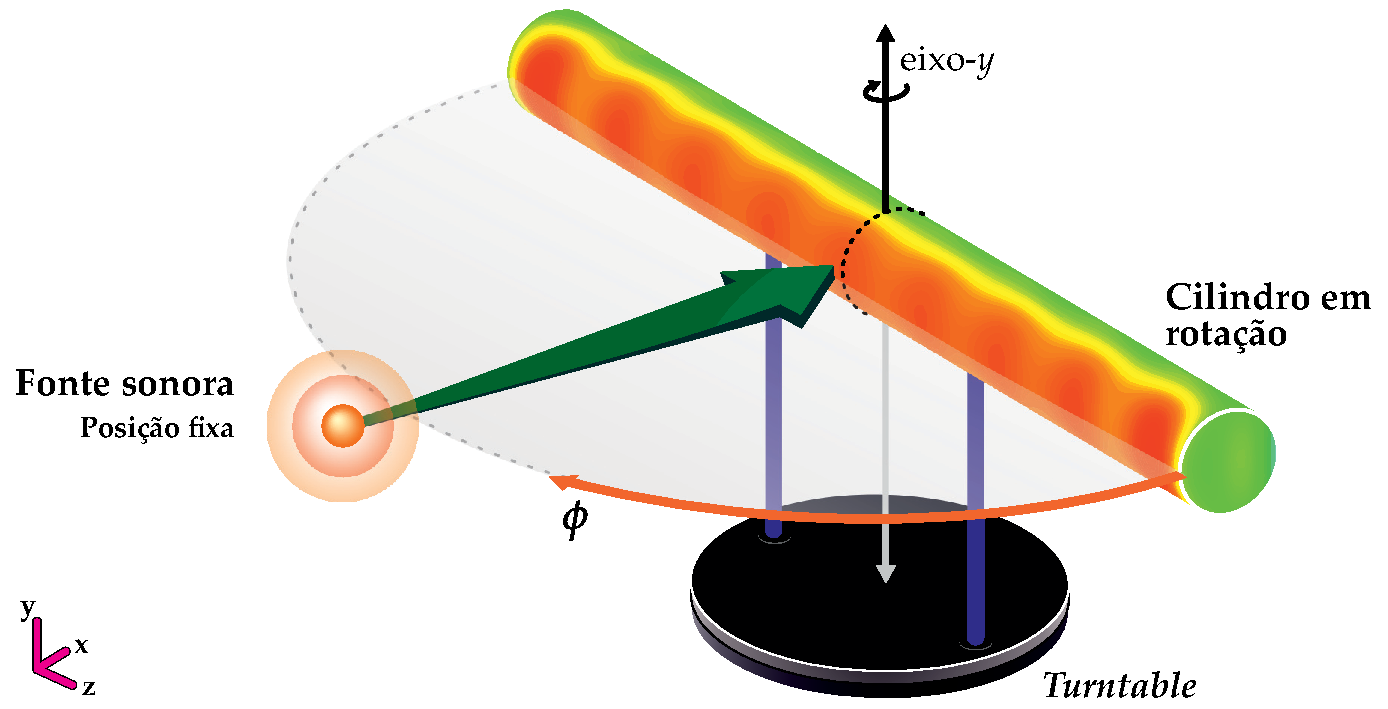
\includegraphics[width=0.72\linewidth]{figs/Measurement-Scheme-Fonseca-2013.pdf}%
	\caption{Medição de \textit{beamforming} com arranjo cilíndrico (adaptado de Fonseca \cite{Fonseca-2013}) --- exemplo de figura.}
	\label{fig:beamforming}%
\end{figure}

\begin{table}[!b]
  \centering \ratb{1.3} 
  \caption{Propriedades microgeométricas e macroscópicas das camadas porosas CPA 1 e CAUQ-B\\ (retirado de Mareze \etal \cite{Mareze-2017}) --- exemplo de tabela.}
	\fontsize{11}{12}\selectfont 
    \begin{tabular}{C{2.9cm} | C{1.5cm} | C{1.5cm} | C{1.5cm} | C{1.5cm} | C{1.5cm} | C{1.0cm}| C{1.0cm}}
    \toprule
		\SetRowColor{LightOrange}
    \textbf{ Amostra / Parâmetro } & $L\txu{p}$ \qquad [$\upmu$\! m] & $L\txu{a}$ \qquad [$\upmu$\! m] & $D\txu{p}$ \qquad [$\upmu$\! m] & $D\txu{a}$ \qquad [$\upmu$\! m] & $\sigma$ [Ns/m\txup{4}] & {$\phi$\quad [--]} & $\alpha_{\infty}$ [--]\\
	  \midrule
		CPA 1 $\Rightarrow$  3,0\% &	1359,81 & 1492,51 & 2344,05 & 1425,67 &	5131 &	0,218 &	1,63\\
		\rowcolor[gray]{.95} CAUQ-B $\Rightarrow$ 4,5\%	& 1598,29 &	701,24 & 2126,46 & 895,34 &	54989 &	0,070 &	2,89\\
    \bottomrule
    \end{tabular}
    \label{tab.exemplo}%
\end{table}%

O rótulo e número das figuras, seguido da legenda, deve aparecer logo abaixo e centralizado (10~pt). Caso utilize figuras de outros autores (ou fontes), mesmo que adaptadas, indique a fonte logo após a legenda descritiva, vide exemplo da Figura~\ref{fig:beamforming}.

O rótulo, número e legenda das tabelas (quadros e códigos também) devem aparecer centralizados na parte superior (vide Tabela~\ref{tab.exemplo}). A fonte das tabelas deve ser apresentada de acordo com a publicação original (quando necessário). A Tabela~\ref{tab.exemplo} apresenta um exemplo do estilo a ser utilizado (o conteúdo da tabela poderá conter tipografia menor que a do texto quando necessário). Ademais, recomenda-se fortemente o sistema de referências cruzadas automatizado. \textbf{Lembre-se que todos os objetos, como figuras e tabelas, devem ser citados no texto.}

\begin{figure}[!ht]
  %\ContinuedFloat %% para continuar a partir da figura anterior
  \centering
	\subfloat[Legenda da Figura~\protect\subref*{fig.figA}.]{\label{fig.figA}
            \makebox[.45\columnwidth]{\includegraphics[height=35mm,page=48]{example-image-duck}} } % makebox ajuda a organizar figs lado a lado
	\quad
  \subfloat[Legenda da Figura~\protect\subref*{fig.figB}.]{\label{fig.figB}
            \makebox[.45\columnwidth]{\includegraphics[height=35mm,page=47]{example-image-duck}} }
  \caption{Exemplo de figuras lado a lado.}
  \label{subfig.exemplo}
\end{figure}


\begin{quadro}[ht!]
%\vspace{-2mm}
  \centering \ratb{1.3} \setlength\aboverulesep{0pt} \setlength\belowrulesep{0pt}
  \caption{Este é um exemplo de um quadro.}
    \fontsize{11}{12}\selectfont 
    \begin{tabular}{| C{2.8cm} | C{1.8cm} | C{1.8cm} |}
    \hline
	\SetRowColor{LightBlue}
    \textbf{ Experimento / Tipo } & \textbf{Exp. 1} & \textbf{Exp. 2}\\
	\midrule
		Tipo 1& Verde & Amarela\\
		\rowcolor[gray]{.95} Tipo 2 & Azul & Branco\\
	\hline
    \end{tabular}
    \label{quad.exemplo}%
    \vspace{2mm}
\end{quadro}%


%% Modelo de figuras lado a lado usando minipage
%\begin{figure*}[b]
    %\centering
    %\begin{minipage}[t]{.48\textwidth}
        %\centering
        %
\includegraphics[width=1\linewidth,page=2]{FIA-logo.pdf}
        %\caption{Figura do lado esquerdo.}
        %\label{fig:ladoE}
    %\end{minipage}%
		%\quad
    %\begin{minipage}[t]{0.48\textwidth}
        %\centering
        %
\includegraphics[width=1\linewidth,page=2]{FIA-logo.pdf}
        %\caption{Figura do lado direito.}
        %\label{fig:ladoD}
    %\end{minipage}
%\end{figure*}

Recomenda-se que gráficos, figuras, fotos e qualquer arquivo gráfico, estejam inseridos no texto em formato .jpg e/ou .png com boa qualidade (ou ainda em formato vetorial em .pdf para usuários do \LaTeX\xspace). Atente para que os elementos de gráficos e figuras sejam legíveis (sobretudo se a informação for pertinente).


A distribuição deste \textit{template} de \LaTeX\xspace inclui o pacote \ttc{Codes2Latex.sty}\footnote{O pacote está ainda em desenvolvimento (sem documentação detalhada), logo, para mais detalhes, consulte o arquivo \ttc{sty}.}, que habilita possibilidades para documentação de códigos genéricos e nas linguagens Matlab, Fortran, Python, LabView e Latex de forma organizada (observe o Código~\ref{code.matlalatex}).

\clearpage
\begin{matlabcode}[Exemplo de um excerto de código (fazendo o Matlab escrever Latex).]{code.matlalatex}
  syms x
  f = taylor(log(1+x));
  latex(f)
\end{matlabcode}

Todos os elementos (figuras e gráficos, por exemplo) podem ser coloridos ou em tons de cinza. Evite a utilização de elementos textuais de outros autores sem a devida citação (e/ou autorização). É essencial que as figuras que apresentarem texto estejam na mesma língua do artigo. Não serão aceitas citações indiretas como \textit{Google Imagens}, por exemplo, assim como recomenda-se evitar o uso de bases de conhecimento voláteis.

\enlargethispage{2mm}

As referências cruzadas devem ser feitas para todos os elementos, por exemplo: Figura~\ref{fig:beamforming} e Tabela~\ref{tab.exemplo} (com apenas a primeira letra maiúscula, evite que exista quebra de linha entre o rótulo e o respectivo número). Caso exista uma subfigura, use Figura~\subref*{fig.figA}, por exemplo.


%%%%%%%%%%%%%%%%%%%%%%%%%%%%%%%%%%%%%%%%%%%%%%%%%%%%%%%%%%%%%%%%%%%%%%%%%%%%%%%%%%%%%%%%%%%%%%%%%%%%%%%%%%%%%%%%%%%
\section{Tipos de artigo}

O evento aceitará \textbf{submissões originais} (isto é, ainda não publicadas) de pesquisas científicas e aplicações de engenharia, arquitetura, áudio, física, matemática, fonoaudiologia e áreas (e subáreas) afins. Assim, serão considerados os seguintes tipos de documento:
%
\begin{itemize}[noitemsep,topsep=0ex] \itemsep=7pt
	\item \textbf{Artigos técnicos e aplicados} (\textit{Technical and applied papers}):
	apresentam material original a partir de aplicações de técnicas conhecidas e/ou em desenvolvimento. Deve apresentar métodos aplicados que estejam de acordo com normativas e/ou que apresentem resultados pertinentes. É essencial que sejam de interesse de pesquisadores e profissionais do tema proposto.
	
	\item \textbf{Artigos científicos} (\textit{Scientific papers}): 
	contém material original (ideias, modelos, experimentos \etc) não publicado, que contribui substancialmente para o avanço da ciência naquele tema. Ele deve estabelecer uma relação entre seu conteúdo e o \textit{estado da arte} já publicado. 

	\item \textbf{Artigos de revisão} (\textit{Review papers}):
	discutem o \textit{estado da arte} sobre o tema pretendido, aclarando desde aspectos básicos até os sofisticados. Esse tipo de submissão deve ser completo no que concerne à literatura, cobrindo em boa parte as ideias, modelos, experimentos \etc já desenvolvidos, mesmo que não estejam de acordo com a opinião do autor. É importante que o assunto seja de interesse da comunidade científica.	
\end{itemize}

\vspace{5pt}

As áreas temáticas do evento incluem:
%	
\begin{itemize}[noitemsep,topsep=-0.25ex] \itemsep=1.5pt
\item[\textbullet] Acústica ambiental;
\item[\textbullet] Acústica da audição e da fala;
\item[\textbullet] Acústica de edificações;
\item[\textbullet] Acústica de salas;
\item[\textbullet] Acústica geral;
\item[\textbullet] Acústica musical;
\item[\textbullet] Acústica submarina;
\item[\textbullet] Acústica subjetiva;
\item[\textbullet] Acústica veicular;
\item[\textbullet] Acústica virtual e técnica biauricular;
\item[\textbullet] Aeroacústica;
\item[\textbullet] Áudio e eletroacústica;
\item[\textbullet] Bioacústica;
\item[\textbullet] Controle de ruído;
\item[\textbullet] Ensino em acústica;
\item[\textbullet] Fonoaudiologia, audiologia e temas relacionados à saúde;
\item[\textbullet] INAD e ações de extensão;
\item[\textbullet] Legislação e normalização em acústica;
\item[\textbullet] Materiais acústicos;
\item[\textbullet] Medições/instrumentação em acústica e vibrações;
\item[\textbullet] Métodos numéricos em acústica e vibrações;
\item[\textbullet] Paisagens sonoras;
\item[\textbullet] Processamento de sinais;
\item[\textbullet] Psicoacústica (acústica fisiológica);
\item[\textbullet] Ruído e vibrações em ambiente laboral;
\item[\textbullet] Técnicas de imageamento acústico;
\item[\textbullet] Ultrassom; e
\item[\textbullet] Vibrações e vibroacústica.
\end{itemize}
	

%%%%%%%%%%%%%%%%%%%%%%%%%%%%%%%%%%%%%%%%%%%%%%%%%%%%%%%%%%%%%%%%%%%%%%%%%%%%%%%%%%%%%%%%%%%%%%%%%%%%%%%%%%%%%%%%%%%
%%%%%%%%%%%%%%%%%%%%%%%%%%%%%%%%%%%%%%%%%%%%%%%%%%%%%%%%%%%%%%%%%%%%%%%%%%%%%%%%%%%%%%%%%%%%%%%%%%%%%%%%%%%%%%%%%%%
\section{Organização do trabalho}

A estrutura do artigo deverá contemplar pelo menos os seguintes itens:
%
\begin{itemize}[noitemsep,topsep=0ex] \itemsep=3pt
	\item Introdução: visão geral sobre o assunto com definição dos objetivos do trabalho, indicando a sua relevância.
	\item Fundamentos: sobretudo em artigos científicos, a fundamentação teórica principal necessária ao entendimento do texto deve ser apresentada e referenciada. 
	\item Desenvolvimento: como o trabalho foi realizado, incluindo detalhes de teoria, materiais e métodos empregados.
	\item Resultados e discussões: parciais ou conclusivos, conforme a modalidade do trabalho, fazendo referência a medições e cálculos estatísticos aplicados, se for o caso.
	\item Conclusões ou Considerações finais: basear-se nas discussões e objetivos, apresentando apontamentos e considerações que findam o estudo/aplicação.
	\item Agradecimentos: opcional, quando for pertinente. Nessa seção admite-se ainda declarações acerca de financiamento de pesquisa/projeto.
	\item Referências: apresentar bibliografia citada no texto.
\end{itemize}
%
Não é preciso necessariamente existir seções com estes nomes. A organização é também dependente do tipo do artigo.
Outros elementos pós-textuais como apêndices são opcionais, desde que eles (no total) não excedam o limite total de 12 páginas. 

%%%%%%%%%%%%%%%%%%%%%%%%%%%%%%%%%%%%%%%%%%%%%%%%%%%%%%%%%%%%%%%%%%%%%%%%%%%%%%%%%%%%%%%%%%%%%%%%%%%%%%%%%%%%%%%%%%%
\subsection{Citações e referências}

Para a confecção das referências deve-se utilizar a norma vigente. As referências devem ser \textbf{numeradas conforme ordem de aparição}, utilizando colchetes \cite{Gomes-2015}. Todas referências devem ser citadas durante o texto. As referências \cite{Mareze-2017,Fonseca-2013,Brandao-2017,Gomes-2015,Oppenheim-2010,Muller-2001,Mareze-2019,aev:piccini2020} deste modelo de artigo são apenas ilustrativas (para efeito de compreensão).

Ao final do documento a seção de referências deve ser colocada. As entradas nela contidas devem ter tipografia com tamanho 10~pt, espaçamento simples e espaçamento de parágrafo de 6~pt. Este \textit{template} de \LaTeX\xspace usa o pacote {\ttfamily abntex2cite} (com melhorias) para a organização das referências. Além disso, recomenda-se a utilização de gerenciadores de banco de dados de bibliografia como o \href{http://www.jabref.org/}{JabRef}, \href{http://www.mendeley.com}{Mendeley} e \href{https://www.zotero.org/}{Zotero}. Em especial para usuários do Word, o Mendeley tem um \textit{plugin} para formatar e inserir as referências no documento .docx.


Dependendo do contexto, o nome do autor pode ou não ser escrito, observe os exemplos a seguir: 
%
\begin{itemize}[noitemsep,topsep=0ex] \itemsep=4pt
	\item 	``... Mareze \etal \cite{Mareze-2019} trabalharam com absorção de materiais porosos...'', ou 
	
	\item ``... para o estudo de acústica de salas \cite{Brandao-2017} recomenda-se a leitura de um livro texto...'', ou
	\item ``... aplicando a Transformada de Fourier nos sinais de entrada \cite{Oppenheim-2010}. '', ou ainda
	\item ``... Fonseca (2013) demonstrou o cálculo de difração para superfícies cilíndricas~\cite{Fonseca-2013}.''
\end{itemize}
%
Todos os autores que constam nas referências devem estar citados no texto.

Em referências com até três autores, por exemplo, Müller e Massarani \cite{Muller-2001}, ambos devem ser citados (quando evocados). No caso de mais de três autores, por exemplo, Gomes \etal \cite{Gomes-2015} deve-se citar somente o último nome do primeiro autor seguido da expressão ``\etal''. Ainda, ao citar mais de uma referência, utilize apenas um colchete, veja alguns exemplos a seguir:
%
\begin{itemize}[noitemsep,topsep=0ex] \itemsep=8pt
	\item ``Trabalhos em temas de acústica e vibrações \cite{Mareze-2017,Fonseca-2013,Brandao-2017}.''
	\item ``Trabalhos em temas de acústica \cite{Mareze-2017,Oppenheim-2010,Muller-2001,sobrac2018:natal, Mareze-2019, jasa:2022eac}.''
	\item ``Trabalhos com análise estatística \cite{Mareze-2017, Brandao-2017, aev:piccini2020}.''
		\item \textbf{Não usar esse estilo:} ``Trabalhos com análise estatística \cite{Mareze-2017}, \cite{Brandao-2017}, \cite{jasa:2022eac} ou \cite{Mareze-2017}--\cite{jasa:2022eac}.''
\end{itemize}
%
Recomenda-se que as referências sejam ordenadas e compactadas (com meia-risca) como em \cite{Mareze-2017,Oppenheim-2010,Muller-2001,Mareze-2019}.

Na seção de referências, sempre que possível, inclua o ISBN, ISSN, DOI\footnote{Para usuários de Latex basta usar o campo ``doi'' de seu repositório \texttt{.bib}.} (com link) e/ou link com a direção online em que o documento citado está disponível.

%%%%%%%%%%%%%%%%%%%%%%%%%%%%%%%%%%%%%%%%%%%%%%%%%%%%%%%%%%%%%%%%%%%%%%%%%%%%%%%%%%%%%%%%%%%%%%%%%%%%%%%%%%%%%%%%%%%
\section{Submissão e avaliação}

Os artigos completos deverão ser enviados pelo sistema próprio do Encontro, disponível no site\linebreak \url{https://www.even3.com.br/sobracnatal2023}, dentro dos prazos estabelecidos. Os autores serão comunicados e receberão o parecer dos avaliadores (em pares) do trabalho. Após atender as correções solicitadas, quando for o caso, o artigo deverá ser reenviado pelo mesmo sistema, seguindo as condições de reenvio. Detalhes acerca de registro autor participante podem ser consultados também no site, ou com a comissão organizadora.

Detalhes acerca de registro do autor participante podem ser consultados também no site, ou com a comissão organizadora.

É responsabilidade dos autores a preparação e envio dos artigos em seu formato final. Por esse motivo, pede-se que verifiquem com atenção a formatação de seus artigos, especialmente gráficos e fotos, quanto à legibilidade e qualidade digital (e para impressão). \textbf{Os artigos deverão ser enviados em formato PDF (com tamanho máximo de 10~Mb).} 

Os metadados do PDF para usuários de \LaTeX\xspace são feitos automaticamente, usuários de MS Word devem conferir no momento da conversão.

% Uso de PDF-a fica opcional.

Em pesquisas que envolvam pessoas (ou seres vivos, em geral), como em acústica subjetiva ou fisiológica, por exemplo, recomenda-se aclarar no artigo o termo de aprovação do Comitê de Ética, caso pertinente.



%%%%%%%%%%%%%%%%%%%%%%%%%%%%%%%%%%%%%%%%%%%%%%%%%%%%%%%%%%%%%%%%%%%%%%%%%%%%%%%%%%%%%%%%%%%%%%%%%%%%%%%%%%%%%%%%%%%
\subsection{Modelos para Word e \LaTeX}

O modelo de \LaTeX\xspace (\texttt{.tex}) foi escrito em codificação UTF8, assim é compatível com Windows, Mac, Linux e \href{https://www.overleaf.com/read/xnhkrtjwprcn}{Overleaf}\footnote{\url{https://www.overleaf.com/read/xnhkrtjwprcn}.}. Pode ser usado livremente para a elaboração dos artigos.

O modelo de \texttt{.docx} foi criado em Microsoft Word 2016 e, com isso, suas funcionalidades de espaçamento e configurações são garantidas para essa versão. Todas eles estão disponíveis com links no \href{https://www.even3.com.br/sobracnatal2023}{site do evento}.

O autor deste texto e dos modelos é o professor William D'Andrea Fonseca, da Engenharia Acústica (EAC) da Universidade Federal de Santa Maria (UFSM).

%%%%%%%%%%%%%%%%%%%%%%%%%%%%%%%%%%%%%%%%%%%%%%%%%%%%%%%%%%%%%%%%%%%%%%%%%%%%%%%%%%%%%%%%%%%%%%%%%%%%%%%%%%%%%%%%%%%
\section{Considerações finais}

Buscou-se, por meio desse \textit{artigo modelo}, elencar e aclarar as instruções para submissão de artigos para o\linebreak XXX~Encontro da Sobrac. 
Este próprio documento pode ser usado como modelo apenas trocando o conteúdo.

%%%%%%%%%%%%%%%%%%%%%%%%%%%%%%%%%%%%%%%%%%%%%%%%%%%%%%%%%%%%%%%%%%%%%%%%%%%%%%%%%%%%%%%%%%%%%%%%%%%%%%%%%%%%%%%%%%%
\section{Agradecimentos}

Se for pertinente, faça agradecimentos.
%
Em caso de trabalhos com fomento, utilize esta seção para elucidar detalhes.

No caso deste documento, gostaríamos de agradecer à cooperação de todos para com o evento.
%%%%%%%%%%%%%%%%%%%%%%%%%%%%%%%%%%%%%%%%%%%%%%%%%%%%%%%%%%%%%%%%%%%%%%%%%%%%%%%%%%%%%%%%%%%%%%%%%%%%%%%%%%%%%%%%%%%
% EOF}         %%% Modelo em português


{\selectlanguage{english}
%%%%%%%%%%%%%%%%%%%%%%%%%%%%%%%%%%%%%%%%%%photos,%%%%%%%%%%%%%%%%%suggested.%%%%%%%%%%%%%%%%%%%%%%%%%%%%%%%%%%%%%%%%%
%%%%%%%%%%%%%%%%%%%%%%%%%%%%%%%%%%%%%%%%%%%%%%%%%%%%%%%%%%%%%%%%%%%%%%%%%%%%%%%%%%%%%%%%%%%%%%%%%%%%%%%%%%%%%%%%%%%%
%%% ARTICLE
%%%%%%%%%%%%%%%%%%Recall%%%%%%%%%%%%%%%%%%%%%%%%%%%%%%%%%%%%%%%%%%%%%%%%%%%%%%%%%%%%%%%%%%%%%%%%%%%%%%%%%%%%%%%%%%
%%%%%%%%%%%%%%%%%%%%%%%%%%%%%%%%%%%%%%%%%%%%%%%%%%%%%%%%%%%%%%%%%%%%%%%%%%%%%%%%%%%%%%%%%%%%%%%%%%%%%%%%%%%%%%%%%%%%
%\clearpage % It is recommended to leave only the abstract data on the first page, although this is not mandatory.

\section{Introduction}

This model instruction text has been developed so that authors can present their articles in a standardized way.
It has been adapted from the template of the \href{https://revista.acustica.org.br}{Acoustics and Vibrations Journal}, for use in the XIII~Ibero-American Congress on Acoustics (FIA 2024).
%
This will provide uniform formatting for the full articles of the event.
This template presents the main guidelines for preparing a complete article in terms of content presentation, graphics, structure, layout, and the procedure for article submission. 
%
This document already includes custom style formatting to help draft the article. Therefore, the author can use this file as a template for this purpose. The templates will be available in Microsoft Word (\texttt{.docx}) and \LaTeX\xspace (\texttt{.tex}). This version is also available on \href{https://www.overleaf.com/read/tjbcfwbtfdtz\#869489}{Overleaf} and \href{https://github.com/willdfonseca/latex}{GitHub} --- and is compatible with Windows, Mac, and Linux. 
%
The authors are responsible for the content, preparation, and submission of the articles according to this template.

The complete text should be single-spaced, using Times New Roman font size 12~pt, and paragraphs with 0~pt spacing before and 6~pt after. It is common practice to write scientific articles in an impersonal tone, so this is recommended. In addition, the articles will be accepted in formal Portuguese, English\footnote{Non-native speakers writing in a foreign language should preferably have their work professionally reviewed.}, and Spanish\footnotemark[2]. 

%%%%%%%%%%%%%%%%%%%%%%%%%%%%%%%%%%%%%%%%%%%%%%%%%%%%%%%%%%%%%%%%%%%%%%%%%%%%%%%%%%%%%%%%%%%%%%%%%%%%%%%%%%%%%%%%%%%
%%%%%%%%%%%%%%%%%%%%%%%%%%%%%%%%%%%%%%%%%%%%%%%%%%%%%%%%%%%%%%%%%%%%%%%%%%%%%%%%%%%%%%%%%%%%%%%%%%%%%%%%%%%%%%%%%%%
\section{Basic guidelines}

This section provides a summary of how the article should be constructed. For more details, refer to the subsequent sections.

\vspace{-8pt}
\begin{enumerate} \itemsep=2pt
    \item The provided LaTeX and Word templates already contain all the configurations described in this document. Additionally, this manuscript provides simultaneous instructions for both text layout platforms.
	\item The first page should contain (for Portuguese and Spanish languages) title, authors, affiliations, abstract, keywords, --- and in English --- \textit{title}, \textit{abstract}, and \textit{keywords}. Submissions in English may contain only authors, affiliations, \textit{title}, \textit{abstract}, and \textit{keywords} (without versions in Portuguese or Spanish).
	\item The text must be written in formal language.
	\item The number of pages must be a minimum of 6 and a maximum of 15, counting from the title page to the end of the references (including appendices, if any).
	\item The paper size is A4, with margins: top 2.0~cm, bottom 2.0~cm, left 1.8~cm, and right 1.8~cm (the spacing between columns is 1.0~cm).
	\item The text should be written in Times New Roman font size 12~pt (as per this template).
	\item The article may contain figures, tables, codes, and equations. If necessary, links may be included in the text. Animations are also accepted, provided they are formatted as figures.
	\item A technical article is understood to have a logical structure, descriptive content, and reproducible results, concluding with references.
\end{enumerate}

%%%%%%%%%%%%%%%%%%%%%%%%%%%%%%%%%%%%%%%%%%%%%%%%%%%%%%%%%%%%%%%%%%%%%%%%%%%%%%%%%%%%%%%%%%%%%%%%%%%%%%%%%%%%%%%%%%%
%%%%%%%%%%%%%%%%%%%%%%%%%%%%%%%%%%%%%%%%%%%%%%%%%%%%%%%%%%%%%%%%%%%%%%%%%%%%%%%%%%%%%%%%%%%%%%%%%%%%%%%%%%%%%%%%%%%
\section{Document and presentation}

Always place text in sections and subsections, do not leave them orphaned (opening a section and proceeding directly to the subsection).

%%%%%%%%%%%%%%%%%%%%%%%%%%%%%%%%%%%%%%%%%%%%%%%%%%%%%%%%%%%%%%%%%%%%%%%%%%%%%%%%%%%%%%%%%%%%%%%%%%%%%%%%%%%%%%%%%%%
\subsection{First page}

The first page should contain the following items provided by the authors: title, authors, affiliations, abstract, keywords, \textit{title}, \textit{abstract}, and \textit{keywords}. 
%
If the complete title is very long, a shorter version is requested to be included in the article's header.

The abstract of the article should be between 150 and 200 words (in 11~pt font). The abstract, keywords, \textit{title}, \textit{abstract}, and \textit{keywords} make up the first page of the article, and it is recommended not to extend to the second page. 
It should provide a concise presentation of the scientific technical article, including an introduction, the objective, a summary of the methodology, the main result, and the main conclusion (preferably in that order). It is not necessary to separate it into items or sections within the abstract. In this way, the reader can grasp the essence of the work. Recall that the abstract is like a movie trailer; people will be interested in reading the entire article if the abstract catches their attention. The abstract should not contain new information not included in the article; undefined abbreviations; prior discussion of other literature; references and citations; and excessive details about the methods used. It is also not the introductory paragraph of the document, which should be placed at the beginning of the text. Use only useful and relevant information, and practice empathy with the potential interested reader. To obtain a cohesive, elegant abstract that aligns with the article, write a draft, complete the document, and, at the end, review it to ensure the content consistently reflects the document's essence. 

Following the abstract, the author should list up to five keywords (avoid using the same words that form the article title). The text of the article should start properly after the \textit{keywords}.

In the authors' affiliations, use numbers as markers, and if there are authors from the same institution, use only one address, and differentiate them by emails. When there are emails from the same domain, try to reduce them using braces \{\}. Use a maximum of two lines for the affiliation of each author from different institutions. See some examples below.
%
\begin{flushleft}
\vspace{-0.25\baselineskip}
\begin{itemize}[topsep=-1ex,align=left,leftmargin=0.2cm] \itemsep=4pt

	\item Fonseca,~W.~D'A.$^1$; Surname,~N.$^2$\\[6pt]	
	$^{1,\,2}$\,Acoustical Engineering Program, Federal University of Santa Maria, Santa Maria, RS, Brazil, 
	 will.fonseca@eac.ufsm.br, name@domain.br.
	
	\item Fonseca,~W.~D'A.$^1$; Mareze,~P.~H.$^2$\\[6pt]	
	$^{1-2}$\,Acoustical Engineering Program, Federal University of Santa Maria, Santa Maria, RS, Brazil,\\
	\{will.fonseca, paulo.mareze\}@eac.ufsm.br.
	
	\item Fonseca,~W.~D'A.$^1$; Surname,~N.$^2$, Mareze,~P.~H.$^3$\\[6pt]	
	$^{1,\,3,\,2}$\,Acoustical Engineering Program, Federal University of Santa Maria, Santa Maria, RS, Brazil,\\
	\{will.fonseca, paulo.mareze\}@eac.ufsm.br, name@domain.br.

	\item Fonseca,~W.~D'A.$^1$; Surname,~N.$^2$\\[6pt]	
	$^{1}$\,Acousticap Engineering Program, Federal University of Santa Maria, Santa Maria, RS, Brazil,
	will.fonseca@eac.ufsm.br.\\[4pt]		
	$^2$\,Laboratory, Institution, City, State, Country, name@domain.br.	
\end{itemize}
\vspace{-0.4\baselineskip}
\end{flushleft}

%%%%%%%%%%%%%%%%%%%%%%%%%%%%%%%%%%%%%%%%%%%%%%%%%%%%%%%%%%%%%%%%%%%%%%%%%%%%%%%%%%%%%%%%%%%%%%%%%%%%%%%%%%%%%%%%%%%
\subsection{Number of pages}

The complete work should contain 6 to 15 pages, counting from the title page to the end of the reference list. Appendices are allowed after the references, provided that they do not exceed 15 pages in total.

To maximize the content on each page, figures, tables, and codes should be presented throughout the body of the text (side-by-side figures are accepted).

%%%%%%%%%%%%%%%%%%%%%%%%%%%%%%%%%%%%%%%%%%%%%%%%%%%%%%%%%%%%%%%%%%%%%%%%%%%%%%%%%%%%%%%%%%%%%%%%%%%%%%%%%%%%%%%%%%%
\subsubsection{Example of a two-level subsection}

This is a two-level subsection for exemplification purposes.

%%%%%%%%%%%%%%%%%%%%%%%%%%%%%%%%%%%%%%%%%%%%%%%%%%%%%%%%%%%%%%%%%%%%%%%%%%%%%%%%%%%%%%%%%%%%%%%%%%%%%%%%%%%%%%%%%%%
\subsection{Page size and margins}

The text should be configured on A4 size paper (210~mm $\times$ 297~mm), in a single column, with distinct numbering for even and odd pages (as in this document). The left and right margins should be 1.8~cm, the bottom 2.0~cm, and the top 2.0~cm. Try to utilize the entire available area. Exceptions can be made, for example, when it is necessary to start a new section, title, subtitle, or caption; these may be allocated at the beginning of the next page.

%%%%%%%%%%%%%%%%%%%%%%%%%%%%%%%%%%%%%%%%%%%%%%%%%%%%%%%%%%%%%%%%%%%%%%%%%%%%%%%%%%%%%%%%%%%%%%%%%%%%%%%%%%%%%%%%%%%
\subsection{Characters and text}

The texts should be written in Times New Roman font. The article title should be on the first page, centered, \textbf{bold}, with only the first letter capitalized (except for proper names), in 18~pt font, and a paragraph spacing of 22~pt afterward. Section titles should be in bold, 12~pt font, with only the first letter capitalized (unless there are proper names), as shown in this template. The subsections should also be in bold, 12~pt font; for both cases, use Times New Roman font. The document text should be single-spaced, 12~pt font, justified, and without indentation in the first line. Avoid using subsections with more than three levels and instead use a list system.

% In LaTeX this is already configured automatically.

Use formal and scientific language in your text\footnote{Footnotes can help clarify details and comments.}. Foreign words should be italicized (for example, as in \textit{instrumentação}). Acronyms, abbreviations, and/or other constructions that are not common knowledge should be explained to the reader, for example, HRTF (\textit{Head-Related Transfer Function}) --- always written upright, including in equations.
Conduct technical and grammatical reviews before submission.

%%%%%%%%%%%%%%%%%%%%%%%%%%%%%%%%%%%%%%%%%%%%%%%%%%%%%%%%%%%%%%%%%%%%%%%%%%%%%%%%%%%%%%%%%%%%%%%%%%%%%%%%%%%%%%%%%%%
\subsection{Line and paragraph spacing}

Single line spacing should be used, as already adopted in this instruction file. For paragraph formatting, choose the justified paragraph option (with 6~pt spacing).

% In LaTeX this is already configured automatically.

%%%%%%%%%%%%%%%%%%%%%%%%%%%%%%%%%%%%%%%%%%%%%%%%%%%%%%%%%%%%%%%%%%%%%%%%%%%%%%%%%%%%%%%%%%%%%%%%%%%%%%%%%%%%%%%%%%%
\subsection{Equations and units}

Units from the International System (SI) will be adopted. When writing your work in Portuguese or Spanish, \textbf{use the comma as the decimal separator} (according to the current Portuguese and Spanish languages), whether in text, tables, figures, and/or graphs. Always strive for consistent precision when comparing numbers, for example: 3.0 is different from 3.00, but has the same precision as 6.0.
If the work is written in English, it is up to the author to use either a period or a comma as the decimal separator (as long as the notations are not mixed).
When writing a number with its unit\footnote{Units are always written ``upright'', i.e., not in italics, for example, 30~N/m$^2$.}, always keep the number together with the corresponding unit, without a line break between them (in MS Word, use Ctrl + Shift + Space [or Alt + 0160], in \LaTeX\xspace use a tilde ($\sim$) between the number and the unit). For example, 3~m separates the input and output and 4,512.28~cm is the measured distance.

Equations should be integrated into the text (in Word, use a simple ``table'') as in the example of Equation~\eqref{eq:area-circ}. They should also be centered and numbered sequentially, with the numbering placed on the right side and in parentheses (see the example). Recall that they are textual elements, so they should be punctuated, and the following text should not normally start with a capital letter. It is recommended to place the nomenclature immediately after the presented variable.

The area of the circle (in m$^2$) is given by
%
\begin{equation}
	A = \pi \, r^2\;,
\label{eq:area-circ}
\end{equation}
%
where $r$ is the radius in meters (m). Remember that variables (like $r$ in this example) are written in \textit{italics} (whether in the equation or the text). However, \textbf{units, functions, and mathematical operators are written ``upright''}, without italics. For example, 32.0~N/m$^2$ was the applied pressure, or
%
\begin{equation}
	\int_a^b p(\phi)\, \dt p\,
\label{eq:int}
\end{equation}
%
was the calculated integral (note that the differential operator ``d'' is upright), for each angle $\phi$ in degrees. Examples of functions include sine, $\sin(\theta)$, or $\log(y)$.

Subscript and superscript text will be in italics only if it corresponds to a relevant variable. If it is a ``complementary name'', the text should be upright, for example, $P\txu{total}$ corresponds to the total pressure in Pa, or $S\txup{tri}$ corresponds to the triangle area in cm$^2$. 
%
However, when referring to a variable, such as $i$, one should write, for example: ``the summation was calculated considering $P_i$ up to the final $i$-th pressure, corresponding to 256''.

If text, acronyms, or units are used in equations, they should be represented upright, for example:
%
\begin{equation}
	\text{density} = \frac{\tx{mass}}{\;\;\tx{volume}\;\;}\,,
\label{eq:density}
\end{equation}
%
where in SI (International System of Units), the unit of density is kilogram per cubic meter (kg/m$^3$).
%
In the text, when it is necessary to cite a previously presented equation, it should be done as follows: Equation~\eqref{eq:density} — with only the first letter capitalized and the corresponding number in parentheses.

%%%%%%%%%%%%%%%%%%%%%%%%%%%%%%%%%%%%%%%%%%%%%%%%%%%%%%%%%%%%%%%%%%%%%%%%%%%%%%%%%%%%%%%%%%%%%%%%%%%%%%%%%%%%%%%%%%%
\subsection{Figures, tables, and codes}

Figures and tables should be inserted within the text, preferably following the paragraphs to which they refer. A mention of figures, tables, and codes in the running text before their presentation is necessary to guide the reader. Figures and tables must contain all the formatting and content elements so that they can be interpreted correctly, without having to resort to the running text to find additional information.  Tables and figures should be separated from the text with \textbf{one (1) blank line} before and after (12~pt).

% In LaTeX this is already configured automatically.

Figures, tables, and codes\footnote{The distribution of this \LaTeX\xspace template includes the \ttc{Codes2Latex.sty} package, which enables possibilities for documenting generic codes and languages such as Matlab, Fortran, Python, LabView, and LaTeX in an organized manner (see Code~\ref{code.matlalatex}) --- the package is still under development.} should be centered and numbered sequentially (see the examples in Figures~\ref{fig:beamforming} and \ref{subfig.exemplo}; Tables~\ref{tab.exemplo} and \ref{quad.exemplo}; and Code~\ref{code.matlalatex}). Strive to use figures and graphs that are entirely comprehensible.

The label and number of the figures, followed by the caption, should appear immediately below and centered (10~pt). If using figures from other authors (or sources), even if adapted, indicate the source immediately after the descriptive caption, as shown in Figure~\ref{fig:beamforming}.

The label, number, and caption of the tables and codes should appear centered at the top (see Table~\ref{tab.exemplo}). The source of the tables should be presented according to the original publication (when necessary). Table~\ref{tab.exemplo} provides an example of the style to be used (the table content may have a smaller font size than the text when necessary). Additionally, the automated cross-referencing system is strongly recommended. \textbf{Remember that all objects, such as figures and tables, must be cited in the text.}

It is recommended that graphics, figures, photos, and any other graphic files are inserted in the text in .jpg and/or .png format with good/adequate quality (or in vector format in .pdf for \LaTeX\xspace users). Make sure that the graphics and pictures are legible (especially if the information is relevant).

\begin{figure}[!ht] %% Example of a figure
	\centering
	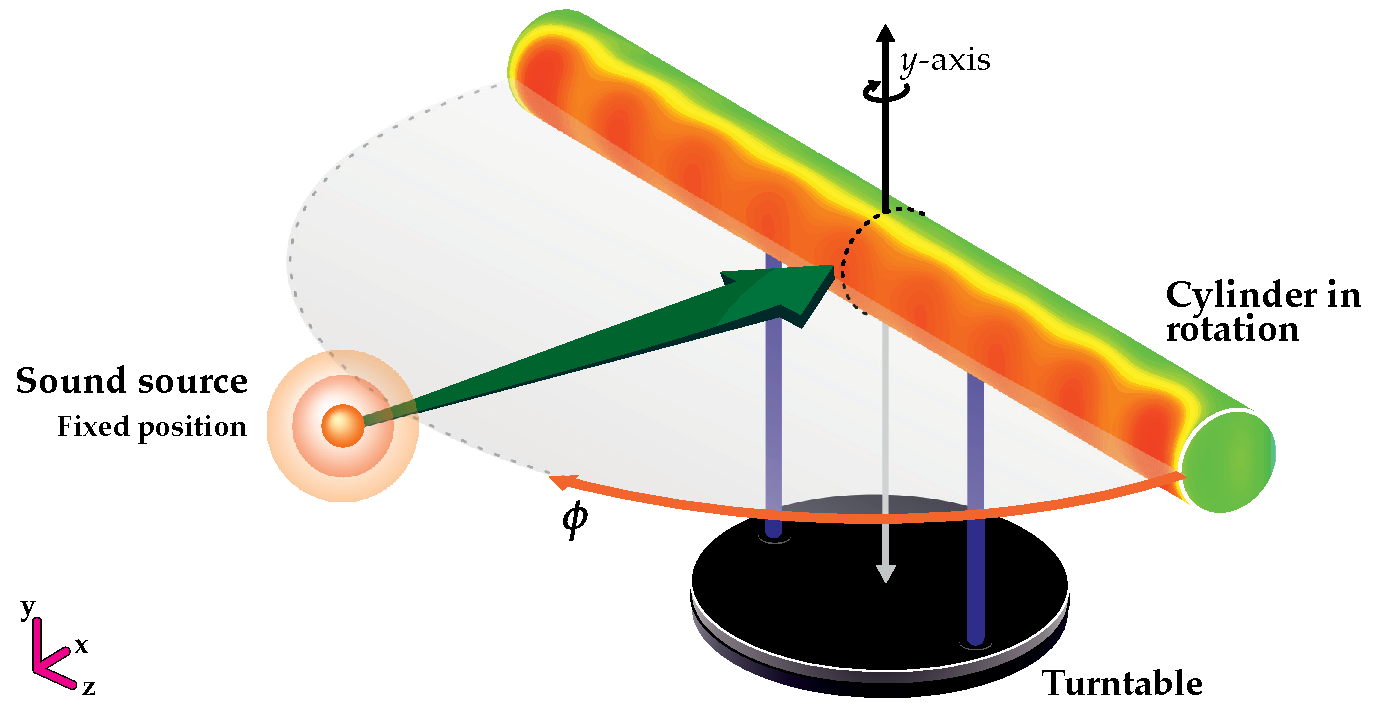
\includegraphics[width=0.70\linewidth]{figs/Measurement-Scheme-Fonseca-2013-en.pdf}%
	\caption{Beamforming measurement with cylindrical array (adapted from Fonseca \cite{Fonseca-2013}) — example of a figure.}
	\label{fig:beamforming}%
\end{figure}

\begin{figure}[!ht]
  %\ContinuedFloat %% to continue from the previous figure
  \centering
	\subfloat[Caption for Figure~\protect\subref*{fig.figA}.]{\label{fig.figA}
            \makebox[.46\columnwidth]{\includegraphics[height=35mm,page=48]{example-image-duck}} } % makebox helps organize side-by-side figures
	\quad
  \subfloat[Caption for Figure~\protect\subref*{fig.figB}.]{\label{fig.figB}
            \makebox[.46\columnwidth]{\includegraphics[height=35mm,page=47]{example-image-duck}} }
  \caption{Example of side-by-side figures.}
  \label{subfig.exemplo}
\end{figure}


\begin{table}[ht!]
%\vspace{-2mm}
  \centering \ratb{1.3} \setlength\aboverulesep{0pt} \setlength\belowrulesep{0pt}
  \caption{This is an example of a table.}
    \fontsize{11}{12}\selectfont 
    \begin{tabular}{| C{2.8cm} | C{1.8cm} | C{1.8cm} |}
    \hline
	\SetRowColor{LightBlue}
    \textbf{ Experiment / Type } & \textbf{Exp. 1} & \textbf{Exp. 2}\\
	\midrule
		Type 1 & Green & Yellow\\
		\rowcolor[gray]{.95} Type 2 & Blue & White\\
	\hline
    \end{tabular}
    \label{quad.exemplo}%
    \vspace{2mm}
\end{table}%

\begin{table}[!htb]
  \centering \ratb{1.3} 
  \caption{Microgeometric and macroscopic properties of porous layers CPA 1 and CAUQ-B\\ (extracted from Mareze \etal \cite{Mareze-2017}) --- example of a table.}
	\fontsize{11}{12}\selectfont 
    \begin{tabular}{C{2.9cm} | C{1.5cm} | C{1.5cm} | C{1.5cm} | C{1.5cm} | C{1.5cm} | C{1.0cm}| C{1.0cm}}
    \toprule
		\SetRowColor{LightOrange}
    \textbf{ Sample / Parameter } & $L\txu{p}$ \qquad [$\upmu$\! m] & $L\txu{a}$ \qquad [$\upmu$\! m] & $D\txu{p}$ \qquad [$\upmu$\! m] & $D\txu{a}$ \qquad [$\upmu$\! m] & $\sigma$ [Ns/m\txup{4}] & {$\phi$\quad [--]} & $\alpha_{\infty}$ [--]\\
	  \midrule
		CPA 1 $\Rightarrow$  3.0\% &	1359.81 & 1492.51 & 2344.05 & 1425.67 &	5131 &	0.218 &	1.63\\
		\rowcolor[gray]{.95} CAUQ-B $\Rightarrow$ 4.5\%	& 1598.29 &	701.24 & 2126.46 & 895.34 &	54989 &	0.070 &	2.89\\
    \bottomrule
    \end{tabular}
    \label{tab.exemplo}%
\end{table}%

%% Example of side-by-side figures using minipage
%\begin{figure}[!htb]
    %\centering
    %\begin{minipage}[t]{.48\textwidth}
        %\centering
        %
\includegraphics[width=1\linewidth,page=2]{FIA-logo.pdf}
        %\caption{Left side figure.}
        %\label{fig:ladoE}
    %\end{minipage}%
		%\quad
    %\begin{minipage}[t]{0.48\textwidth}
        %\centering
        %
\includegraphics[width=1\linewidth,page=2]{FIA-logo.pdf}
        %\caption{Right side figure.}
        %\label{fig:ladoD}
    %\end{minipage}
%\end{figure}

\begin{matlabcode}[Example of a code snippet (making Matlab write LaTeX).]{code.matlalatex}
  syms x
  f = taylor(log(1+x));
  latex(f)
\end{matlabcode}

All elements (such as figures and graphs) can be in color or grayscale. Avoid using textual elements from other authors without proper citation (and/or authorization). Figures containing text are essential to be in the same language as the article. Avoid indirect citations such as \textit{Google Images}, and avoid using volatile knowledge bases.

Cross-references should be made for all elements, for example: Figure~\ref{fig:beamforming} and Table~\ref{tab.exemplo} (with only the first letter capitalized, avoid line breaks between the label and the respective number). If there is a subfigure, use Figure~\subref*{fig.figA}, for example.


%%%%%%%%%%%%%%%%%%%%%%%%%%%%%%%%%%%%%%%%%%%%%%%%%%%%%%%%%%%%%%%%%%%%%%%%%%%%%%%%%%%%%%%%%%%%%%%%%%%%%%%%%%%%%%%%%%%
\section{Types of articles}

The event will accept \textbf{original submissions} (i.e., not yet published) of scientific research and applications in engineering, architecture, audio, physics, mathematics, speech therapy, and related areas (and subareas). Thus, the following types of documents are suggested:
%
\begin{itemize}[topsep=0ex] \itemsep=2pt
	\item \textbf{Technical and applied papers}:
	present original material from applications of known and/or developing techniques. They should describe applied methods that comply with standards and/or present relevant results. It is essential that these articles interest researchers and professionals in the proposed area.
	
	\item \textbf{Scientific papers}: 
	include original (ideas, models, experiments, \etc) unpublished material that significantly contributes to the advancement of scientific knowledge in the addressed topic. The content should establish a connection with the existing state-of-the-art in the published literature.

	\item \textbf{Review papers}:
	discuss the state-of-the-art on the subject in question, elucidating from basic concepts to more complex aspects. This type of submission should be comprehensive regarding the existing literature, broadly covering ideas, models, experiments, \etc, already developed, even if they disagree with the author's view. It is crucial that the topic is of interest to the scientific community.
\end{itemize}

\vspace{5pt}

The thematic areas of the event include:
%	
\begin{enumerate}[topsep=0ex] \itemsep=0.0pt
    \item Acoustics Education
    \item Architectural and Building Acoustics
    \item Biomedical Acoustics and Bioacoustics
    \item Computational Acoustics
		\vspace{-0.25em}
    \begin{enumerate}[noitemsep,topsep=0ex] 
        \item Acoustic Imaging and Virtual Acoustics/Auralization
    \end{enumerate}
    \item Environmental, Industrial, and Occupational Noise
    \item Forensic Acoustics
    \item Musical Acoustics
    \item Physical Acoustics and Ultrasound
		\vspace{-0.25em}
    \begin{enumerate}[noitemsep,topsep=0ex]
        \item Structured Metamaterials for Noise and Vibration Control
    \end{enumerate}
    \item Professional Audio and Electroacoustics
    \item Psychological and Physiological Acoustics
    \item Signal Processing in Acoustics
    \item Soundscapes and Ecoacoustics
    \item Structural Acoustics and Vibrations
    \item Underwater Acoustics
\end{enumerate}

	
%%%%%%%%%%%%%%%%%%%%%%%%%%%%%%%%%%%%%%%%%%%%%%%%%%%%%%%%%%%%%%%%%%%%%%%%%%%%%%%%%%%%%%%%%%%%%%%%%%%%%%%%%%%%%%%%%%%
%%%%%%%%%%%%%%%%%%%%%%%%%%%%%%%%%%%%%%%%%%%%%%%%%%%%%%%%%%%%%%%%%%%%%%%%%%%%%%%%%%%%%%%%%%%%%%%%%%%%%%%%%%%%%%%%%%%
\section{Article organization}

The article/work should be structured; therefore, the following items are suggested.
%
\begin{itemize}[noitemsep,topsep=0ex] \itemsep=3pt
	\item Introduction: an overview of the subject with the definition of the work's objectives, indicating its relevance.
	\item Fundamentals: especially in scientific articles, the main theoretical foundation necessary for understanding the text should be presented and referenced.
	\item Development: how the work was carried out, including details of the theory, materials, and methods used.
	\item Results and discussions: partial or conclusive, depending on the type of work, referring to measurements and applied statistical calculations, if applicable.
	\item Conclusions (or Final Considerations): based on discussions and objectives, presenting remarks and considerations that conclude the study/application.
	\item Acknowledgments: optional, when pertinent. In this section, statements about research/project funding are also admitted.
	\item References: present the bibliographic references cited in the text.
\end{itemize}
%
It is not necessarily required to have sections with these same names. The organization also depends on the type of article.
Other post-textual elements, such as the appendices, are optional.

%%%%%%%%%%%%%%%%%%%%%%%%%%%%%%%%%%%%%%%%%%%%%%%%%%%%%%%%%%%%%%%%%%%%%%%%%%%%%%%%%%%%%%%%%%%%%%%%%%%%%%%%%%%%%%%%%%%
\subsection{Citations and references}

References should follow the current standard. References must be \textbf{numbered in order of appearance}, using square brackets \cite{Gomes-2015}. All references should be cited throughout the text. The references \cite{Mareze-2017,Fonseca-2013,Brandao-2017,Gomes-2015,Oppenheim-2010,Muller-2001,Mareze-2019,aev:piccini2020} in this article template are for illustrative purposes only.

The reference section should be placed at the end of the document. The entries should have a font size of 10~pt, single line spacing, and paragraph spacing of 6~pt. This \LaTeX\xspace template uses the {\ttfamily natbib} package for organizing references. In addition, it is recommended to use bibliography database managers such as \href{http://www.jabref.org/}{JabRef}, \href{http://www.mendeley.com}{Mendeley}, and \href{https://www.zotero.org/}{Zotero}. Especially for Word users, Mendeley has a plugin to format and insert references into the.docx document.

Depending on the context, the author's name may or may not be written. Observe the following examples:
%
\begin{itemize}[noitemsep,topsep=0ex] \itemsep=4pt
	\item 	``... Mareze \etal \cite{Mareze-2019} worked with the absorption of porous materials...'', or 
	\item ``... for the study of room acoustics \cite{Brandao-2017} it is recommended to read a textbook...'', or
	\item ``... applying the Fourier Transform to input signals \cite{Oppenheim-2010}.'', or 
	\item ``... \txtcite{Fonseca-2013} demonstrated the calculation of diffraction for cylindrical surfaces~\cite{Fonseca-2013}.''
\end{itemize}
%
All authors listed in the references must be cited in the text.

For references with up to three authors, for example, Müller and Massarani \cite{Muller-2001}, both should be cited (when mentioned). In the case of more than three authors, for example, Gomes \etal \cite{Gomes-2015}, only the last name of the first author followed by the expression ``\etal'' should be cited. Additionally, when citing more than one reference, use only one bracket. See some examples below.
%
\begin{itemize}[noitemsep,topsep=0ex] \itemsep=8pt
	\item ``Works on acoustics and vibrations topics \cite{Mareze-2017,Fonseca-2013,Brandao-2017}.''
	\item ``Works on acoustics topics \cite{Mareze-2017,Oppenheim-2010,Muller-2001,Mareze-2019, jasa:2022eac}.''
	%\item ``Works with statistical analysis \cite{Mareze-2017, Brandao-2017, aev:piccini2020}.''
	\item \textbf{Do not use this style:} ``Works with statistical analysis \cite{Mareze-2017}, \cite{Brandao-2017}, \cite{jasa:2022eac} or \cite{Mareze-2017}--\cite{jasa:2022eac}.''
\end{itemize}
%
References should be ordered and compacted (with a hyphen) as in \cite{Mareze-2017,Oppenheim-2010,Muller-2001,Mareze-2019}.
%
In the reference section, whenever possible, include ISBN, ISSN, DOI\footnote{For LaTeX users, simply use the "doi" field of your \texttt{.bib} repository.} (with link), and/or a link to the online location where the cited document is available.

%%%%%%%%%%%%%%%%%%%%%%%%%%%%%%%%%%%%%%%%%%%%%%%%%%%%%%%%%%%%%%%%%%%%%%%%%%%%%%%%%%%%%%%%%%%%%%%%%%%%%%%%%%%%%%%%%%%
\section{Submission of articles}

Complete articles should be submitted through the congress's system, available on the website\linebreak \url{https://www.fia2024.cl}, within the established deadlines. Details regarding participant author registration can also be found on the event website or with the organizing committee.

Authors are responsible for the preparation and submission of articles in their final format. Therefore, it is requested that they carefully check the formatting of their articles, especially graphs and photos, for legibility and digital (and print) quality. \textbf{Articles should be submitted in PDF format (with a maximum size of 16~Mb).}

% PDF metadata for LaTeX users is automatically done; MS Word users should check during the conversion.

% The use of PDF-a is optional.

% For research involving people (or living beings in general), such as in subjective or physiological acoustics, it is recommended to clarify the Ethics Committee approval term in the article, if applicable.

%%%%%%%%%%%%%%%%%%%%%%%%%%%%%%%%%%%%%%%%%%%%%%%%%%%%%%%%%%%%%%%%%%%%%%%%%%%%%%%%%%%%%%%%%%%%%%%%%%%%%%%%%%%%%%%%%%%
\subsection{Templates for Word and \LaTeX}

The \LaTeX\xspace template (\texttt{.tex}) was written in UTF8 encoding, making it compatible with Windows, Mac, Linux, and \href{https://www.overleaf.com/read/tjbcfwbtfdtz\#869489}{Overleaf}\footnote{\url{https://www.overleaf.com/read/tjbcfwbtfdtz\#869489}.}. It can be freely used for article preparation.

The \texttt{.docx} template was created in Microsoft Word 2016, ensuring that its spacing and configuration functionality are guaranteed for that version. All templates are available through links on the \href{https://www.fia2024.cl}{event website} (or \href{https://github.com/willdfonseca/latex}{this repository}).

The author of this text and the templates is Professor William D'Andrea Fonseca, from the Acoustical Engineering Program (EAC) at the Federal University of Santa Maria (UFSM), Brazil.

%%%%%%%%%%%%%%%%%%%%%%%%%%%%%%%%%%%%%%%%%%%%%%%%%%%%%%%%%%%%%%%%%%%%%%%%%%%%%%%%%%%%%%%%%%%%%%%%%%%%%%%%%%%%%%%%%%%
\section{Final considerations}

The purpose of this \textit{article template} is to list and clarify the guidelines for submitting papers to the XIII~Ibero-American Congress of Acoustics. This document serves as a practical guide and can be used as a template by replacing its content as necessary.

%%%%%%%%%%%%%%%%%%%%%%%%%%%%%%%%%%%%%%%%%%%%%%%%%%%%%%%%%%%%%%%%%%%%%%%%%%%%%%%%%%%%%%%%%%%%%%%%%%%%%%%%%%%%%%%%%%%
\section{Acknowledgments}

If relevant, include acknowledgments here.
%
For funded work, use this section to clarify the details.

% In the case of this document, we would like to thank everyone's cooperation for the event.

%%%%%%%%%%%%%%%%%%%%%%%%%%%%%%%%%%%%%%%%%%%%%%%%%%%%%%%%%%%%%%%%%%%%%%%%%%%%%%%%%%%%%%%%%%%%%%%%%%%%%%%%%%%%%%%%%%%
% EOF
}        %%% Template in English


% {\selectlanguage{spanish}
% %%%%%%%%%%%%%%%%%%%%%%%%%%%%%%%%%%%%%%%%%%%%%%%%%%%%%%%%%%%%%%%%%%%%%%%%%%%%%%%%%%%%%%%%%%%%%%%%%%%%%%%%%%%%%%%%%%%%
%%%%%%%%%%%%%%%%%%%%%%%%%%%%%%%%%%%%%%%%%%%%%%%%%%%%%%%%%%%%%%%%%%%%%%%%%%%%%%%%%%%%%%%%%%%%%%%%%%%%%%%%%%%%%%%%%%%%
%%% ARTÍCULO
%%%%%%%%%%%%%%%%%%%%%%%%%%%%%%%%%%%%%%%%%%%%%%%%%%%%%%%%%%%%%%%%%%%%%%%%%%%%%%%%%%%%%%%%%%%%%%%%%%%%%%%%%%%%%%%%%%%%
%%%%%%%%%%%%%%%%%%%%%%%%%%%%%%%%%%%%%%%%%%%%%%%%%%%%%%%%%%%%%%%%%%%%%%%%%%%%%%%%%%%%%%%%%%%%%%%%%%%%%%%%%%%%%%%%%%%%
%\clearpage % Se recomienda dejar solo los datos del resumen en la primera página, sin embargo, esto no es obligatorio.

\section{Introducción}

Este texto de instrucciones modelo ha sido elaborado para que los autores puedan presentar los artículos de forma estandarizada.
%
Se ha adaptado del modelo de la \href{https://revista.acustica.org.br}{Revista Acústica y Vibraciones}, siendo de uso para el XIII~Congreso Iberoamericano de Acústica (FIA 2024).
Esto proporcionará una uniformidad en el formateo de los artículos completos del evento.
En este modelo se presentan las principales directrices para la elaboración del artículo completo en lo que respecta a la presentación de contenido, gráfica, estructura, diagramación y al procedimiento para la presentación de los artículos.
%
Este documento ya cuenta con el formateo de estilos personalizados para la elaboración del artículo. El autor puede, por lo tanto, utilizar este archivo como modelo para esa finalidad. Se pondrán a disposición modelos (\textit{templates}) en Microsoft Word (\texttt{.docx}) y \LaTeX\xspace (\texttt{.tex}). Esta versión también está disponible en \href{https://www.overleaf.com/read/tjbcfwbtfdtz\#869489}{Overleaf} y en \href{https://github.com/willdfonseca/latex}{GitHub} --- siendo aún compatible con Windows, Mac y Linux.
Los autores son responsables del contenido, elaboración y envío de los artículos de acuerdo con el presente modelo.

El texto completo deberá estar en interlineado simple, tipografía Times New Roman tamaño 12~pt y párrafo con espaciado de 0~pt antes y 6~pt después. Es práctica común la escritura de artículos científicos en impersonal, por lo tanto, esto es recomendable. Además, se aceptarán en lengua culta\footnote{Haga uso de correctores ortográficos y/o de gramática, tanto Ms Word como Overleaf los poseen, se indica además el uso de otras herramientas como el \href{https://languagetool.org/es}{Language Tool}.} portuguesa, inglesa\footnote{Artículos en lengua extranjera escritos por no nativos deben, preferentemente, recibir revisión profesional.} y española\footnotemark[2].


%%%%%%%%%%%%%%%%%%%%%%%%%%%%%%%%%%%%%%%%%%%%%%%%%%%%%%%%%%%%%%%%%%%%%%%%%%%%%%%%%%%%%%%%%%%%%%%%%%%%%%%%%%%%%%%%%%%
%%%%%%%%%%%%%%%%%%%%%%%%%%%%%%%%%%%%%%%%%%%%%%%%%%%%%%%%%%%%%%%%%%%%%%%%%%%%%%%%%%%%%%%%%%%%%%%%%%%%%%%%%%%%%%%%%%%
\section{Orientaciones básicas}

En esta sección hay un resumen de cómo debe construirse el artículo. Para más detalles, consulte las secciones subsecuentes.

\vspace{-8pt}
\begin{enumerate} \itemsep=2pt
    \item Los modelos en LaTeX y Word proporcionados ya contienen todas las configuraciones descritas en este documento. Además, este manuscrito proporciona simultáneamente instrucciones para las dos plataformas de diagramación de texto.
	\item La primera página debe contener (para las lenguas portuguesa y española) título, autores, afiliaciones, resumen, palabras clave, \textit{title}, \textit{abstract} y \textit{keywords}. Las presentaciones en inglés pueden contener solo autores, afiliaciones, \textit{title}, \textit{abstract} y \textit{keywords} (sin versiones en portugués o español).
	\item El texto debe estar escrito en lengua culta vigente.
	\item El número de páginas debe ser como mínimo 6 y como máximo 15, contando desde la página que contiene el título, hasta el final de las referencias (incluyendo apéndices, si los hay).
	\item El tamaño del papel es A4, con márgenes: superior de 2,0~cm, inferior de 2,0~cm, izquierda de 1,8~cm y derecha de 1,8~cm (el espaciado entre columnas es de 1,0~cm).
	\item El texto debe estar escrito con tipografía Times New Roman con tamaño 12~pt (conforme a este modelo).
	\item El artículo puede contener figuras, tablas, cuadros, códigos y ecuaciones. En el texto, si es necesario, se pueden colocar enlaces. También se aceptan animaciones, siempre y cuando estén diagramadas como figuras.
	\item Se entiende que un artículo técnico tenga una estructura lógica, descriptiva y contenido susceptible de reproducción, concluyendo en las referencias del trabajo.
\end{enumerate}


%%%%%%%%%%%%%%%%%%%%%%%%%%%%%%%%%%%%%%%%%%%%%%%%%%%%%%%%%%%%%%%%%%%%%%%%%%%%%%%%%%%%%%%%%%%%%%%%%%%%%%%%%%%%%%%%%%%
%%%%%%%%%%%%%%%%%%%%%%%%%%%%%%%%%%%%%%%%%%%%%%%%%%%%%%%%%%%%%%%%%%%%%%%%%%%%%%%%%%%%%%%%%%%%%%%%%%%%%%%%%%%%%%%%%%%
\section{Documento y presentación}

Siempre coloque texto en secciones y subsecciones, no las deje huérfanas (abriendo una sección y pasando directamente a la subsección).

%%%%%%%%%%%%%%%%%%%%%%%%%%%%%%%%%%%%%%%%%%%%%%%%%%%%%%%%%%%%%%%%%%%%%%%%%%%%%%%%%%%%%%%%%%%%%%%%%%%%%%%%%%%%%%%%%%%
\subsection{Primera página}

La primera página debe contener los siguientes elementos colocados por los autores: título, autores, afiliaciones, resumen, palabras clave, \textit{title}, \textit{abstract} y \textit{keywords}.
%
En caso de que el título completo sea muy extenso, se solicita una versión corta para que sea incluida en el encabezado de las páginas del artículo.

El resumen del artículo podrá tener entre 150 y 200 palabras (en tipografía de 11~pt). El resumen, las palabras clave, \textit{title}, \textit{abstract} y \textit{keywords} constituyen la primera página del artículo; se recomienda no extenderse a la segunda página.
Debe hacer una presentación concisa del artículo técnico-científico, conteniendo una introducción, el objetivo, una síntesis de la metodología, el principal resultado y la principal conclusión (preferiblemente en ese orden). No es necesario separar en ítems o secciones dentro del resumen. Así, el lector puede conocer la esencia del trabajo. Recuerde que el resumen es como el \textit{tráiler} de una película; las personas estarán interesadas en leer completamente el artículo si el resumen les interesa. El resumen no debe contener información nueva no incluida en el artículo; abreviaturas indefinidas; discusión previa de otra literatura; referencias y citas y exceso de detalles sobre los métodos empleados. Tampoco es el párrafo de introducción del documento; esto debe colocarse al inicio del texto. Utilice solo información útil y relevante; haga un ejercicio de empatía con el posible lector interesado. Para obtener un resumen cohesionado, elegante y acorde al artículo, escriba una previa, realice la escritura completa del documento y, al final, revíselo observando si su contenido refleja de manera consistente el contenido del documento.

Siguiendo el resumen, el autor debe listar hasta cinco palabras clave (evite colocar las mismas palabras que forman el título del artículo). El texto del artículo debe comenzar propiamente después de los \textit{keywords}.

En la afiliación de los autores use números como marcas y en caso de que existan autores de una misma institución, utilice solo una dirección y los diferencie en los correos electrónicos. Cuando existan correos electrónicos de un mismo dominio, procure reducir usando llaves \{\}. Utilice un máximo de dos líneas para la afiliación de cada autor de instituciones diferentes. A continuación se presentan algunos ejemplos:
%
\begin{flushleft}
\vspace{-0.25\baselineskip}
\begin{itemize}[topsep=-1ex,align=left,leftmargin=0.2cm] \itemsep=4pt

	\item Fonseca,~W.~D'A.$^1$; Apellido,~N.$^2$\\[6pt]	
	$^{1,\,2}$\,Ingeniería Acústica, Universidad Federal de Santa María, Santa María, RS, Brasil,
	will.fonseca@eac.ufsm.br, nombre@dominio.br.
	
	\item Fonseca,~W.~D'A.$^1$; Mareze,~P.~H.$^2$\\[6pt]	
	$^{1-2}$\,Ingeniería Acústica, Universidad Federal de Santa María, Santa María, RS, Brasil,\\
	\{will.fonseca, paulo.mareze\}@eac.ufsm.br.
	
	\item Fonseca,~W.~D'A.$^1$; Apellido,~N.$^2$; Mareze,~P.~H.$^3$\\[6pt]	
	$^{1,\,3,\,2}$\,Ingeniería Acústica, Universidad Federal de Santa María, Santa María, RS, Brasil,\\
	\{will.fonseca, paulo.mareze\}@eac.ufsm.br, nombre@dominio.br.

	\item Fonseca,~W.~D'A.$^1$; Apellido,~N.$^2$\\[6pt]	
	$^{1}$\,Ingeniería Acústica, Universidad Federal de Santa María, Santa María, RS, Brasil,
	will.fonseca@eac.ufsm.br.\\[4pt]		
	$^2$\,Laboratorio, Institución, Ciudad, Estado, País, nombre@dominio.br.	
\end{itemize}
\vspace{-0.4\baselineskip}
\end{flushleft}


%%%%%%%%%%%%%%%%%%%%%%%%%%%%%%%%%%%%%%%%%%%%%%%%%%%%%%%%%%%%%%%%%%%%%%%%%%%%%%%%%%%%%%%%%%%%%%%%%%%%%%%%%%%%%%%%%%%
\subsection{Número de páginas}

El trabajo completo debe contener de 6 a 15 páginas, contando desde la página que contiene el título y el final de la lista de referencias. Se admiten apéndices, después de las referencias, siempre y cuando no excedan las 15 páginas en total.

Como forma de optimizar al máximo el contenido de cada página, las figuras, tablas, cuadros y códigos deben ser presentados a lo largo del cuerpo del texto (se aceptan figuras lado a lado).

%%%%%%%%%%%%%%%%%%%%%%%%%%%%%%%%%%%%%%%%%%%%%%%%%%%%%%%%%%%%%%%%%%%%%%%%%%%%%%%%%%%%%%%%%%%%%%%%%%%%%%%%%%%%%%%%%%%
\subsubsection{Ejemplo de subsección de dos niveles}

Esta es una subsección de dos niveles a modo de ejemplo.

%%%%%%%%%%%%%%%%%%%%%%%%%%%%%%%%%%%%%%%%%%%%%%%%%%%%%%%%%%%%%%%%%%%%%%%%%%%%%%%%%%%%%%%%%%%%%%%%%%%%%%%%%%%%%%%%%%%
\subsection{Tamaño de la hoja y márgenes}

El texto debe configurarse en hoja de tamaño A4 (210~mm $\times$ 297~mm), en una columna, con numeración distinta en páginas pares e impares (como está en este documento). Las márgenes izquierda y derecha deberán tener 1,8~cm, la inferior 2,0~cm y la superior 2,0~cm. Procure utilizar toda el área disponible. Se pueden admitir excepciones, por ejemplo, cuando sea necesario comenzar una nueva sección, título, subtítulo o leyenda: estos podrán ubicarse al inicio de la página siguiente.

%%%%%%%%%%%%%%%%%%%%%%%%%%%%%%%%%%%%%%%%%%%%%%%%%%%%%%%%%%%%%%%%%%%%%%%%%%%%%%%%%%%%%%%%%%%%%%%%%%%%%%%%%%%%%%%%%%%
\subsection{Caracteres y texto}

Los textos deberán estar escritos en tipografía Times New Roman. El título del artículo deberá estar en la primera página, centrado, \textbf{en negritas}, con solo la primera letra en mayúscula (excepto nombres propios), cuerpo 18~pt y párrafo con espacio de 22~pt después. Los títulos de las secciones deberán estar en negritas, cuerpo 12~pt, con solo la primera letra en mayúscula (a menos que existan nombres propios), según se presenta en este modelo. Las subsecciones deben estar también en negritas, cuerpo 12~pt, para ambos casos, utilice tipografía Times New Roman. El texto del documento debe tener interlineado simple, cuerpo 12~pt, justificado y sin sangría en la primera línea. Evite el uso de subsecciones con más de tres niveles y, para ello, intente usar un sistema de listas.

% En Latex esto ya está configurado automáticamente.

Utilice lenguaje culto y científico en su texto\footnote{Las notas al pie pueden ayudar a aclarar detalles y comentarios.}. Las palabras extranjeras deberán escribirse en cursivas (por ejemplo, como en \textit{proceedings}). Siglas, acrónimos, abreviaturas y/u otras construcciones que escapan al conocimiento común deben ser presentadas al lector, por ejemplo, HRTF (\textit{Head-Related Transfer Function}) --- siempre se escriben sin inclinación, incluso en ecuaciones. Realice revisiones gramaticales y de contenido técnico antes de la presentación.

%%%%%%%%%%%%%%%%%%%%%%%%%%%%%%%%%%%%%%%%%%%%%%%%%%%%%%%%%%%%%%%%%%%%%%%%%%%%%%%%%%%%%%%%%%%%%%%%%%%%%%%%%%%%%%%%%%%
\subsection{Espaciado entre líneas y párrafos}

Debe emplearse interlineado simple, como ya se ha adoptado en este archivo de instrucciones.
En el formateo de los párrafos elija la opción de párrafo justificado (con espaciado de 6~pt).

% En Latex esto ya está configurado automáticamente.

%%%%%%%%%%%%%%%%%%%%%%%%%%%%%%%%%%%%%%%%%%%%%%%%%%%%%%%%%%%%%%%%%%%%%%%%%%%%%%%%%%%%%%%%%%%%%%%%%%%%%%%%%%%%%%%%%%%
\subsection{Ecuaciones y unidades}

Se adoptarán las unidades del Sistema Internacional (SI). Al escribir su trabajo en portugués o español, en los números, \textbf{use el separador decimal coma} (conforme al idioma portugués y español vigente), ya sea en el texto, tablas, figuras y/o gráficos, además de buscar siempre el uso de una misma precisión al comparar números, por ejemplo: 3,0 es diferente de 3,00, pero tiene la misma precisión que 6,0.
En caso de que el trabajo esté escrito en inglés, queda a criterio del autor usar punto o coma como separador decimal (siempre que no se mezclen las notaciones).
Al escribir un número con su unidad\footnote{Las unidades siempre se escriben sin inclinación, es decir, no en cursivas, por ejemplo, 30~N/m$^2$.}, mantenga siempre el número junto a la unidad correspondiente, sin que exista un salto de línea entre ellos (en Ms Word use Ctrl + Shift + Espacio [o Alt + 0160], en \LaTeX\xspace coloque una tilde ($\sim$) entre el número y la unidad). Por ejemplo, 3~m de distancia separa la entrada y la salida y 4.512,28~cm es la distancia medida.

Las ecuaciones deberán estar intercaladas con el texto (en Word use una ``tabla'' simple) conforme al ejemplo de la Ecuación~\eqref{eq:area-circ}. Deberán estar centradas y numeradas secuencialmente, con la numeración colocada en el lado derecho y entre paréntesis (véase ejemplo). Recuerde que son elementos textuales, por lo tanto, deben ser puntuadas y el texto siguiente normalmente no debe comenzar con letra mayúscula. Se recomienda colocar la nomenclatura inmediatamente después de la variable presentada.

El área del círculo (en m$^2$) está dada por
%
\begin{equation}
	A = \pi \, r^2\;,
\label{eq:area-circ}
\end{equation}
%
en que $r$ es el radio en metros (m). Recuerde que las variables (como $r$ en este ejemplo) se escriben en \textit{cursivas} (ya sea en la ecuación o en el texto). Sin embargo, \textbf{unidades, funciones y operadores matemáticos se escriben ``sin inclinación''}, sin aplicar cursivas. Por ejemplo, 32,0~N/m$^2$ fue la presión aplicada, o también
%
\begin{equation}
	\int_a^b p(\phi)\, \dt p\,
\label{eq:int}
\end{equation}
%
fue la integral calculada (observe que el operador diferencial ``d'' está sin inclinación), para cada ángulo $\phi$ en grados. Como funciones, se puede citar el seno, $\sen(\theta)$, o también $\log(y)$, por ejemplo.

El texto subíndice y superíndice solo será en cursivas si corresponde a alguna variable pertinente. Si es un ``nombre complementario'', el texto debe colocarse sin formato cursivo, por ejemplo, $P\txu{total}$ corresponde a la presión total en Pa, o también $S\txup{tri}$ corresponde al área del triángulo en cm$^2$.
Sin embargo, al referirse a una variable, como $i$, debe escribirse, por ejemplo: ``la suma se calculó considerando $P_i$ hasta la $i$-ésima presión final, correspondiente a 256''.

Si texto, siglas o unidades son utilizados en ecuaciones, su representación debe ser sin inclinación, por ejemplo:
%
\begin{equation}
	\text{densidad} = \frac{\tx{masa}}{\;\;\tx{volumen}\;\;}\,,
\label{eq:densidad}
\end{equation}
%
siendo que en el SI (Sistema Internacional de Unidades) la unidad de densidad es el kilogramo por metro cúbico (kg/m$^3$).
En el texto, cuando sea necesario citar una ecuación ya presentada, debe hacerse de la siguiente manera: Ecuación~\eqref{eq:densidad} --- con solo la primera letra en mayúscula y con el número correspondiente entre paréntesis.

%%%%%%%%%%%%%%%%%%%%%%%%%%%%%%%%%%%%%%%%%%%%%%%%%%%%%%%%%%%%%%%%%%%%%%%%%%%%%%%%%%%%%%%%%%%%%%%%%%%%%%%%%%%%%%%%%%%
\subsection{Figuras, tablas, cuadros y códigos}

Las figuras y tablas deben ser insertadas durante el texto, preferiblemente a continuación de los párrafos a los que se refieren. Es necesario hacer una mención a las figuras, tablas, cuadros y códigos en el texto corrido, antes de su presentación, para la orientación del lector. Las figuras, tablas y cuadros deben contener todos los elementos de formato y contenido para que sean interpretados correctamente, sin necesidad de recurrir al texto corrido para buscar información adicional. Se debe separar del texto las tablas y figuras con \textbf{una (1) línea} en blanco antes y después (12~pt).

% En Latex esto ya está configurado automáticamente.

Las figuras, tablas, cuadros y códigos\footnote{La distribución de este \textit{template} de \LaTeX\xspace incluye el paquete \ttc{Codes2Latex.sty}, que habilita posibilidades para documentación de códigos genéricos y en los lenguajes Matlab, Fortran, Python, LabView y Latex de forma organizada (vea el Código~\ref{code.matlalatex}) --- el paquete está aún en desarrollo.} deberán estar centrados y numerados secuencialmente (vea el ejemplo en las Figuras~\ref{fig:beamforming} y \ref{subfig.exemplo}; Tabla~\ref{tab.exemplo}; Cuadro~\ref{quad.exemplo} y Código~\ref{code.matlalatex}). Busque utilizar figuras y gráficos en los que su contenido pueda ser completamente comprendido.

El rótulo y número de las figuras, seguido de la leyenda, deben aparecer justo debajo y centrados (10~pt). Si utiliza figuras de otros autores (o fuentes), aunque estén adaptadas, indique la fuente justo después de la leyenda descriptiva, vea el ejemplo de la Figura~\ref{fig:beamforming}.

El rótulo, número y leyenda de las tablas (cuadros y códigos también) deben aparecer centrados en la parte superior (vea la Tabla~\ref{tab.exemplo}). La fuente de las tablas debe ser presentada de acuerdo con la publicación original (cuando sea necesario). La Tabla~\ref{tab.exemplo} presenta un ejemplo del estilo a ser utilizado (el contenido de la tabla podrá tener una tipografía menor que la del texto cuando sea necesario). Además, se recomienda encarecidamente el sistema de referencias cruzadas automatizado. \textbf{Recuerde que todos los objetos, como figuras y tablas, deben ser citados en el texto.}

Se recomienda que gráficos, figuras, fotos y cualquier archivo gráfico, estén insertados en el texto en formato .jpg y/o .png con buena calidad (o incluso en formato vectorial en .pdf para usuarios de \LaTeX\xspace). Asegúrese de que los elementos de gráficos y figuras sean legibles (sobre todo si la información es pertinente).

\begin{figure}[!ht] %% Ejemplo de figura
	\centering
	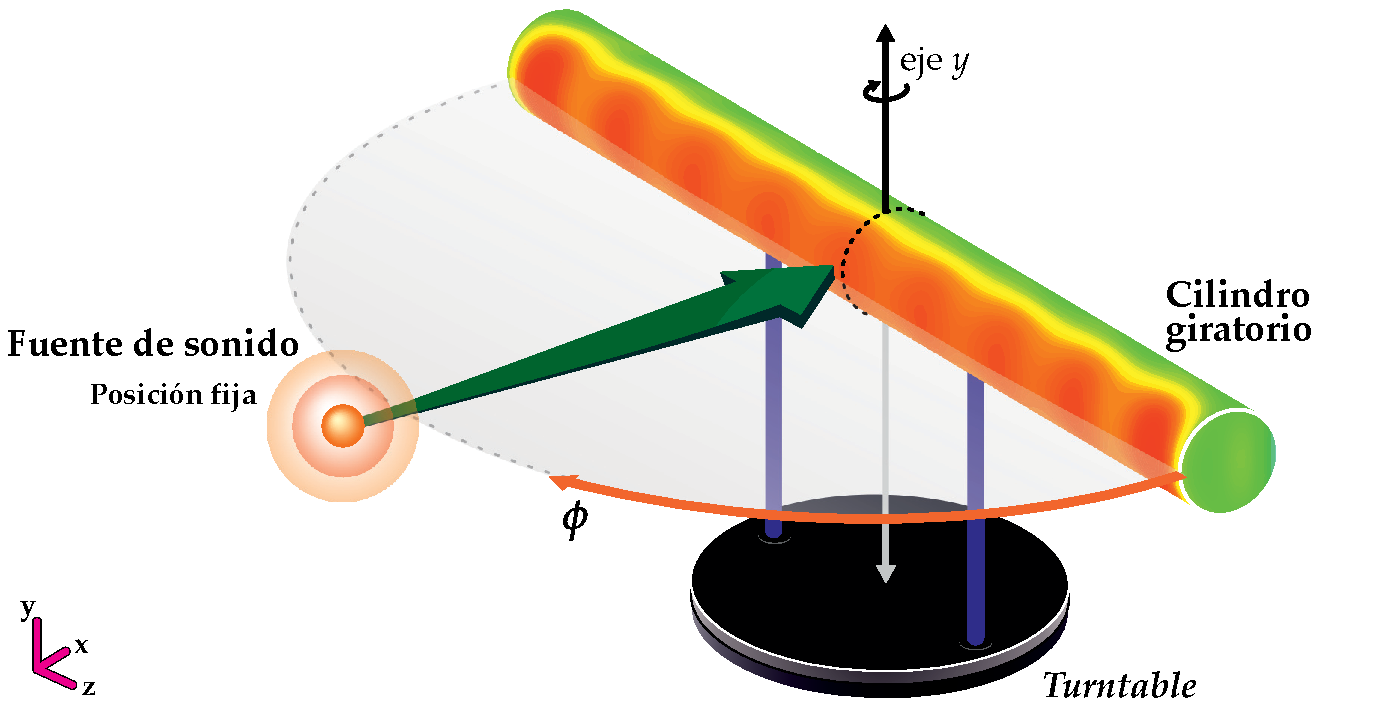
\includegraphics[width=0.72\linewidth]{figs/Measurement-Scheme-Fonseca-2013-sp.pdf}%
	\caption{Medición de \textit{beamforming} con arreglo cilíndrico (adaptado de Fonseca \cite{Fonseca-2013}) --- ejemplo de figura.}
	\label{fig:beamforming}%
\end{figure}


\begin{figure}[!ht]
  %\ContinuedFloat %% para continuar a partir de la figura anterior
  \centering
	\subfloat[Leyenda de la Figura~\protect\subref*{fig.figA}.]{\label{fig.figA}
            \makebox[.46\columnwidth]{\includegraphics[height=35mm,page=48]{example-image-duck}} } % makebox ayuda a organizar figs lado a lado
	\quad
  \subfloat[Leyenda de la Figura~\protect\subref*{fig.figB}.]{\label{fig.figB}
            \makebox[.46\columnwidth]{\includegraphics[height=35mm,page=47]{example-image-duck}} }
  \caption{Ejemplo de figuras lado a lado.}
  \label{subfig.exemplo}
\end{figure}


\begin{cuadro}[ht!] % En español
%\vspace{-2mm}
  \centering \ratb{1.3} \setlength\aboverulesep{0pt} \setlength\belowrulesep{0pt}
  \caption{Este es un ejemplo de un cuadro.}
    \fontsize{11}{12}\selectfont 
    \begin{tabular}{| C{2.8cm} | C{1.8cm} | C{1.8cm} |}
    \hline
	\SetRowColor{LightBlue}
    \textbf{ Experimento / Tipo } & \textbf{Exp. 1} & \textbf{Exp. 2}\\
	\midrule
		Tipo 1 & Verde & Amarilla\\
		\rowcolor[gray]{.95} Tipo 2 & Azul & Blanco\\
	\hline
    \end{tabular}
    \label{quad.exemplo}%
    \vspace{2mm}
\end{cuadro}%


\begin{table}[!htb]
  \centering \ratb{1.3} 
  \caption{Propiedades microgeométricas y macroscópicas de las capas porosas CPA 1 y CAUQ-B\\ (extraído de Mareze \etal \cite{Mareze-2017}) --- ejemplo de tabla.}
	\fontsize{11}{12}\selectfont 
    \begin{tabular}{C{2.9cm} | C{1.5cm} | C{1.5cm} | C{1.5cm} | C{1.5cm} | C{1.5cm} | C{1.0cm}| C{1.0cm}}
    \toprule
		\SetRowColor{LightOrange}
    \textbf{ Muestra / Parámetro } & $L\txu{p}$ \qquad [$\upmu$\! m] & $L\txu{a}$ \qquad [$\upmu$\! m] & $D\txu{p}$ \qquad [$\upmu$\! m] & $D\txu{a}$ \qquad [$\upmu$\! m] & $\sigma$ [Ns/m\txup{4}] & {$\phi$\quad [--]} & $\alpha_{\infty}$ [--]\\
	  \midrule
		CPA 1 $\Rightarrow$  3,0\% &	1359,81 & 1492,51 & 2344,05 & 1425,67 &	5131 &	0,218 &	1,63\\
		\rowcolor[gray]{.95} CAUQ-B $\Rightarrow$ 4,5\%	& 1598,29 &	701,24 & 2126,46 & 895,34 &	54989 &	0,070 &	2,89\\
    \bottomrule
    \end{tabular}
    \label{tab.exemplo}%
\end{table}%


%% Modelo de figuras lado a lado usando minipage
%\begin{figure*}[b]
    %\centering
    %\begin{minipage}[t]{.48\textwidth}
        %\centering
        %
\includegraphics[width=1\linewidth,page=2]{FIA-logo.pdf}
        %\caption{Figura del lado izquierdo.}
        %\label{fig:ladoE}
    %\end{minipage}%
		%\quad
    %\begin{minipage}[t]{0.48\textwidth}
        %\centering
        %
\includegraphics[width=1\linewidth,page=2]{FIA-logo.pdf}
        %\caption{Figura del lado derecho.}
        %\label{fig:ladoD}
    %\end{minipage}
%\end{figure*}


\begin{matlabcode}[Ejemplo de un extracto de código (haciendo que Matlab escriba Latex).]{code.matlalatex}
  syms x
  f = taylor(log(1+x));
  latex(f)
\end{matlabcode}

Todos los elementos (figuras y gráficos, por ejemplo) pueden ser en color o en tonos de gris. Evite la utilización de elementos textuales de otros autores sin la debida citación (y/o autorización). Es esencial que las figuras que presenten texto estén en el mismo idioma del artículo. Evite citas indirectas como \textit{Google Imágenes}, por ejemplo, así como se recomienda evitar el uso de bases de conocimiento volátiles.

Las referencias cruzadas deben hacerse para todos los elementos, por ejemplo: Figura~\ref{fig:beamforming} y Tabla~\ref{tab.exemplo} (con solo la primera letra en mayúscula, evite que haya un salto de línea entre el rótulo y el número correspondiente). Si existe una subfigura, use Figura~\subref*{fig.figA}, por ejemplo.

%%%%%%%%%%%%%%%%%%%%%%%%%%%%%%%%%%%%%%%%%%%%%%%%%%%%%%%%%%%%%%%%%%%%%%%%%%%%%%%%%%%%%%%%%%%%%%%%%%%%%%%%%%%%%%%%%%%
\section{Tipos de artículo}

El evento aceptará \textbf{envíos originales} (es decir, aún no publicados) de investigaciones científicas y aplicaciones de ingeniería, arquitectura, audio, física, matemáticas, terapia del lenguaje y áreas (y subáreas) afines. Así, se sugieren los siguientes tipos de documentos:
%
\begin{itemize}[topsep=0ex] \itemsep=2pt
	\item \textbf{Artículos técnicos y aplicados} (\textit{Technical and applied papers}):
	presentan material original a partir de aplicaciones de técnicas conocidas y/o en desarrollo. Deben describir métodos aplicados que estén en conformidad con normativas y/o que presenten resultados relevantes. Es fundamental que estos artículos despierten el interés de investigadores y profesionales en el área propuesta.
	
	\item \textbf{Artículos científicos} (\textit{Scientific papers}): 
	incluyen material original (ideas, modelos, experimentos, etc.) inédito, que contribuye significativamente al avance del conocimiento científico en el tema abordado. El contenido debe establecer una conexión con el \textit{estado del arte} existente en la literatura publicada.

	\item \textbf{Artículos de revisión} (\textit{Review papers}):
	abordan el \textit{estado del arte} sobre el tema en cuestión, elucidando desde conceptos básicos hasta aspectos más complejos. Este tipo de envío debe ser exhaustivo en relación a la literatura existente, cubriendo ampliamente ideas, modelos, experimentos, etc., ya desarrollados, aunque discrepen de la visión del autor. Es crucial que el tema sea de interés para la comunidad científica.
\end{itemize}

\vspace{5pt}

Las áreas temáticas del evento incluyen:
%	
\begin{enumerate}[topsep=0ex] \itemsep=0.0pt
    \item Acústica Arquitectónica y de la Edificación
    \item Acústica Biomédica y Bioacústica
    \item Acústica Computacional
    \vspace{-0.25em}
    \begin{enumerate}[noitemsep,topsep=0ex] 
        \item Imágenes acústicas y acústica virtual/auralización
    \end{enumerate}    
    \item Acústica Estructural y Vibraciones
    \item Acústica Física y Ultrasonidos
    \vspace{-0.25em}
    \begin{enumerate}[noitemsep,topsep=0ex]
        \item Metamateriales estructurados para el control de ruido y vibraciones
    \end{enumerate}    
    \item Acústica Forense
    \item Acústica Musical
    \item Acústica Psicológica y Fisiológica
    \item Acústica Subacuática
    \item Audio Profesional y Electroacústica
    \item Educación en Acústica
    \item Paisajes Sonoros y Ecoacústica
    \item Procesado de Señales en Acústica
    \item Ruido Ambiental, Industrial y Ocupacional
\end{enumerate}


%%%%%%%%%%%%%%%%%%%%%%%%%%%%%%%%%%%%%%%%%%%%%%%%%%%%%%%%%%%%%%%%%%%%%%%%%%%%%%%%%%%%%%%%%%%%%%%%%%%%%%%%%%%%%%%%%%%
%%%%%%%%%%%%%%%%%%%%%%%%%%%%%%%%%%%%%%%%%%%%%%%%%%%%%%%%%%%%%%%%%%%%%%%%%%%%%%%%%%%%%%%%%%%%%%%%%%%%%%%%%%%%%%%%%%%
\section{Organización del trabajo}

El trabajo debe estar estructurado; por lo tanto, se sugieren los siguientes ítems:
%
\begin{itemize}[noitemsep,topsep=0ex] \itemsep=3pt
	\item Introducción: visión general sobre el tema con definición de los objetivos del trabajo, indicando su relevancia.
	\item Fundamentos: sobre todo en artículos científicos, la fundamentación teórica principal necesaria para la comprensión del texto debe ser presentada y referenciada.
	\item Desarrollo: cómo se realizó el trabajo, incluyendo detalles de teoría, materiales y métodos empleados.
	\item Resultados y discusiones: parciales o conclusivos, según la modalidad del trabajo, haciendo referencia a mediciones y cálculos estadísticos aplicados, si es el caso.
	\item Conclusiones (o Consideraciones finales): basarse en las discusiones y objetivos, presentando apuntes y consideraciones que finalizan el estudio/aplicación.
	\item Agradecimientos: opcional, cuando sea pertinente. En esta sección se admiten también declaraciones sobre financiamiento de investigación/proyecto.
	\item Referencias: presentar las referencias bibliográficas citadas en el texto.
\end{itemize}
%
No es necesario que existan secciones con estos nombres. La organización también depende del tipo de artículo.
Otros elementos post-textuales como apéndices son opcionales.


%%%%%%%%%%%%%%%%%%%%%%%%%%%%%%%%%%%%%%%%%%%%%%%%%%%%%%%%%%%%%%%%%%%%%%%%%%%%%%%%%%%%%%%%%%%%%%%%%%%%%%%%%%%%%%%%%%%
\subsection{Citas y referencias}

Para la confección de las referencias se debe utilizar la norma vigente. Las referencias deben ser \textbf{numeradas conforme al orden de aparición}, utilizando corchetes \cite{Gomes-2015}. Todas las referencias deben ser citadas en el texto. Las referencias \cite{Mareze-2017,Fonseca-2013,Brandao-2017,Gomes-2015,Oppenheim-2010,Muller-2001,Mareze-2019,aev:piccini2020} de este modelo de artículo son solo ilustrativas (para efecto de comprensión).

Al final del documento se debe incluir la sección de referencias. Las entradas en esta sección deben tener tipografía con tamaño 10~pt, espaciado simple y espaciado de párrafo de 6~pt. Esta plantilla de \LaTeX\xspace usa el paquete {\ttfamily natbib} para la organización de las referencias. Además, se recomienda la utilización de gestores de bases de datos bibliográficas como \href{http://www.jabref.org/}{JabRef}, \href{http://www.mendeley.com}{Mendeley} y \href{https://www.zotero.org/}{Zotero}. En especial para usuarios de Word, Mendeley tiene un \textit{plugin} para formatear e insertar las referencias en el documento .docx.

Dependiendo del contexto, el nombre del autor puede o no ser escrito, observe algunos ejemplos a continuación:
%
\begin{itemize}[noitemsep,topsep=0ex] \itemsep=4pt
	\item 	``... Mareze \etal \cite{Mareze-2019} trabajaron con absorción de materiales porosos...'', o 
	
	\item ``... para el estudio de acústica de salas \cite{Brandao-2017} se recomienda la lectura de un libro de texto...'', o
	\item ``... aplicando la Transformada de Fourier en las señales de entrada \cite{Oppenheim-2010}. '', o también
	\item ``... \txtcite{Fonseca-2013} demostró el cálculo de difracción para superficies cilíndricas~\cite{Fonseca-2013}.''
\end{itemize}
%
Todos los autores que figuran en las referencias deben estar citados en el texto.

En referencias con hasta tres autores, por ejemplo, Müller y Massarani \cite{Muller-2001}, ambos deben ser citados (cuando sean mencionados). En el caso de más de tres autores, por ejemplo, Gomes \etal \cite{Gomes-2015}, se debe citar solo el último nombre del primer autor seguido de la expresión ``\etal''. Además, al citar más de una referencia, utilice solo un corchete, vea algunos ejemplos a continuación:
%
\begin{itemize}[noitemsep,topsep=0ex] \itemsep=8pt
	\item ``Trabajos en temas de acústica y vibraciones \cite{Mareze-2017,Fonseca-2013,Brandao-2017}.''
	\item ``Trabajos en temas de acústica \cite{Mareze-2017,Oppenheim-2010,Muller-2001, Mareze-2019, jasa:2022eac}.''
	%\item ``Trabajos con análisis estadístico \cite{Mareze-2017, Brandao-2017, aev:piccini2020}.''
	\item \textbf{No usar este estilo:} ``Trabajos con análisis estadístico \cite{Mareze-2017}, \cite{Brandao-2017}, \cite{jasa:2022eac} o \cite{Mareze-2017}--\cite{jasa:2022eac}.''
\end{itemize}
%
Se recomienda que las referencias sean ordenadas y compactadas (con guion) como en \cite{Mareze-2017,Oppenheim-2010,Muller-2001,Mareze-2019}.
%
En la sección de referencias, siempre que sea posible, incluya el ISBN, ISSN, DOI\footnote{Para usuarios de Latex basta usar el campo ``doi'' de su repositorio \texttt{.bib}.} (con enlace) y/o enlace con la dirección en línea donde el documento citado está disponible.

%%%%%%%%%%%%%%%%%%%%%%%%%%%%%%%%%%%%%%%%%%%%%%%%%%%%%%%%%%%%%%%%%%%%%%%%%%%%%%%%%%%%%%%%%%%%%%%%%%%%%%%%%%%%%%%%%%%
\section{Envío de artículos}

Los artículos completos deberán ser enviados por el sistema propio del congreso, disponible en el sitio web\linebreak \url{https://www.fia2024.cl}, dentro de los plazos establecidos. Detalles acerca del registro de autor participante pueden consultarse también en el sitio del evento o con la comisión organizadora.

Es responsabilidad de los autores la preparación y envío de los artículos en su formato final. Por este motivo, se pide que verifiquen con atención la formateo de sus artículos, especialmente gráficos y fotos, en cuanto a la legibilidad y calidad digital (y para impresión). \textbf{Los artículos deberán ser enviados en formato PDF (con tamaño máximo de 16~Mb).}

%Los metadatos del PDF para usuarios de \LaTeX\xspace se generan automáticamente, usuarios de MS Word deben verificar en el momento de la conversión.

%El uso de PDF-a es opcional.

%En investigaciones que involucren personas (o seres vivos en general), como en acústica subjetiva o fisiológica, por ejemplo, se recomienda aclarar en el artículo el término de aprobación del Comité de Ética, si es pertinente.


%%%%%%%%%%%%%%%%%%%%%%%%%%%%%%%%%%%%%%%%%%%%%%%%%%%%%%%%%%%%%%%%%%%%%%%%%%%%%%%%%%%%%%%%%%%%%%%%%%%%%%%%%%%%%%%%%%%
\subsection{Modelos para Word y \LaTeX}

El modelo de \LaTeX\xspace (\texttt{.tex}) fue escrito en codificación UTF8, por lo tanto, es compatible con Windows, Mac, Linux y \href{https://www.overleaf.com/read/tjbcfwbtfdtz\#869489}{Overleaf}\footnote{\url{https://www.overleaf.com/read/tjbcfwbtfdtz\#869489}.}. Puede ser usado libremente para la elaboración de los artículos.

El modelo de \texttt{.docx} fue creado en Microsoft Word 2016 y, con ello, sus funcionalidades de espaciado y configuraciones están garantizadas para esa versión. Todos ellos están disponibles con enlaces en el \href{https://www.fia2024.cl}{sitio del evento} (o \href{https://github.com/willdfonseca/latex}{en este repositorio}).

El autor de este texto y de los modelos es el profesor William D'Andrea Fonseca, de Ingeniería Acústica (EAC) de la Universidad Federal de Santa María (UFSM), Brasil.

%%%%%%%%%%%%%%%%%%%%%%%%%%%%%%%%%%%%%%%%%%%%%%%%%%%%%%%%%%%%%%%%%%%%%%%%%%%%%%%%%%%%%%%%%%%%%%%%%%%%%%%%%%%%%%%%%%%
\section{Consideraciones finales}

Este \textit{artículo modelo} tuvo como objetivo enumerar y esclarecer las directrices para el envío de trabajos al XIII~Congreso Iberoamericano de Acústica. Este documento sirve como una guía práctica, pudiendo ser utilizado como modelo al reemplazar su contenido según sea necesario.


%%%%%%%%%%%%%%%%%%%%%%%%%%%%%%%%%%%%%%%%%%%%%%%%%%%%%%%%%%%%%%%%%%%%%%%%%%%%%%%%%%%%%%%%%%%%%%%%%%%%%%%%%%%%%%%%%%%
\section{Agradecimientos}

Si es pertinente, haga agradecimientos.
%
En caso de trabajos con financiamiento, utilice esta sección para aclarar detalles.

%En el caso de este documento, nos gustaría agradecer la cooperación de todos para con el evento.

%%%%%%%%%%%%%%%%%%%%%%%%%%%%%%%%%%%%%%%%%%%%%%%%%%%%%%%%%%%%%%%%%%%%%%%%%%%%%%%%%%%%%%%%%%%%%%%%%%%%%%%%%%%%%%%%%%%
% EOF
}       %%% Modelo en español

%%%%%%%%%%%%%%%%%%%%%%%%%%%%%%%%%%%%%%%%%%%%%%%%%%%%%%%%%%%%%%%%%%%%%%%%%%%%%%%%%%%%%%%%%%%%%%%%%%%%%%%%%%%%%%%%%%%%
%%%%%%%%%%%%%%%%%%%%%%%%%%%%%%%%%%%%%%%%%%%%%%%%%%%%%%%%%%%%%%%%%%%%%%%%%%%%%%%%%%%%%%%%%%%%%%%%%%%%%%%%%%%%%%%%%%%%
%%% Referências || References
\renewcommand{\refname}{\RefsName} \addcontentsline{toc}{section}{\refname} 

% \bibliographystyle{unsrtnat-br} %% Para artigo em português
% \bibliographystyle{unsrtnat-sp} %% Para artíclo en español
\bibliographystyle{unsrtnat-en} %% For article in english

{\footnotesize 
% \bibliography{biblio/bibliografia-br}
% \bibliography{biblio/bibliografia-sp}
\bibliography{biblio/bibliografia-en}
}
%%%%%%%%%%%%%%%%%%%%%%%%%%%%%%%%%%%%%%%%%%%%%%%%%%%%%%%%%%%%%%%%%%%%%%%%%%%%%%%%%%%%%%%%%%%%%%%%%%%%%%%%%%%%%%%%%%%
%%%%%%%%%%%%%%%%%%%%%%%%%%%%%%%%%%%%%%%%%%%%%%%%%%%%%%%%%%%%%%%%%%%%%%%%%%%%%%%%%%%%%%%%%%%%%%%%%%%%%%%%%%%%%%%%%%%
%%%%%%%%%%%%%%%%%%%%%%%%%%%%%%%%%%%%%%%%%%%%%%%%%%%%%%%%%%%%%%%%%%%%%%%%%%%%%%%%%%%%%%%%%%%%%%%%%%%%%%%%%%%%%%%%%%%
%%% Apêndice
%%%%%%%%%%%%%%%%%%%%%%%%%%%%%%%%%%%%%%%%%%%%%%%%%%%%%%%%%%%%%%%%%%%%%%%%%%%%%%%%%%%%%%%%%%%%%%%%%%%%%%%%%%%%%%%%%%%
% \appendix
% \section{Exemplo de apêndice}

% Este é um exemplo de apêndice, geralmente se colocam informações adicionais ou derivações produzidas pelos autores.

%% Este modelo (\textit{template} de \LaTeX) tem alguns comandos adicionais que facilitam a escrita, como, por exemplo, \lcode{\\F} (\F\xspace) para simbolizar a Transformada de Fourier. Para conhecer melhor os comandos, consulte o arquivo \texttt{FIA2024.sty}.

%%%%%%%%%%%%%%%%%%%%%%%%%%%%%%%%%%%%%%%%%%%%%%%%%%%%%%%%%%%%%%%%%%%%%%%%%%%%%%%%%%%%%%%%%%%%%%%%%%%%%%%%%%%%%%%%%%%
%%%%%%%%%%%%%%%%%%%%%%%%%%%%%%%%%%%%%%%%%%%%%%%%%%%%%%%%%%%%%%%%%%%%%%%%%%%%%%%%%%%%%%%%%%%%%%%%%%%%%%%%%%%%%%%%%%%
%\section{Escrevendo um código de apêndice}
%
% Caso existam códigos muito extensos, o apêndice pode ser convertido para uma coluna, como exemplificado nesta seção com o Código~\ref{code.fc}.
%
%\inputcodeLatin{Matlab}{Exemplo de inclusão de código (de Matlab) em duas colunas.}{code.fc}{FC.m}

%%%%%%%%%%%%%%%%%%%%%%%%%%%%%%%%%%%%%%%%%%%%%%%%%%%%%%%%%%%%%%%%%%%%%%%%%%%%%%%%%%%%%%%%%%%%%%%%%%%%%%%%%%%%%%%%%%%
%%%%%%%%%%%%%%%%%%%%%%%%%%%%%%%%%%%%%%%%%%%%%%%%%%%%%%%%%%%%%%%%%%%%%%%%%%%%%%%%%%%%%%%%%%%%%%%%%%%%%%%%%%%%%%%%%%%
%%% Español
% \appendix
% \section{Ejemplo de apéndice}

% Este es un ejemplo de apéndice, generalmente se colocan informaciones adicionales o derivaciones producidas por los autores.

%% Este modelo (\textit{template} de \LaTeX) tiene algunos comandos adicionales que facilitan la escritura, como, por ejemplo, \lcode{\\F} (\F\xspace) para simbolizar la Transformada de Fourier. Para conocer mejor los comandos, consulte el archivo \texttt{FIA2024.sty}.

%%%%%%%%%%%%%%%%%%%%%%%%%%%%%%%%%%%%%%%%%%%%%%%%%%%%%%%%%%%%%%%%%%%%%%%%%%%%%%%%%%%%%%%%%%%%%%%%%%%%%%%%%%%%%%%%%%%
%%%%%%%%%%%%%%%%%%%%%%%%%%%%%%%%%%%%%%%%%%%%%%%%%%%%%%%%%%%%%%%%%%%%%%%%%%%%%%%%%%%%%%%%%%%%%%%%%%%%%%%%%%%%%%%%%%%
%\section{Escribiendo un código de apéndice}
%
% Si existen códigos muy extensos, el apéndice puede ser convertido a una columna, como se ejemplifica en esta sección con el Código~\ref{code.fc}.
%
%\inputcodeLatin{Matlab}{Ejemplo de inclusión de código (de Matlab) en dos columnas.}{code.fc}{FC.m}

%%%%%%%%%%%%%%%%%%%%%%%%%%%%%%%%%%%%%%%%%%%%%%%%%%%%%%%%%%%%%%%%%%%%%%%%%%%%%%%%%%%%%%%%%%%%%%%%%%%%%%%%%%%%%%%%%%%
%%%%%%%%%%%%%%%%%%%%%%%%%%%%%%%%%%%%%%%%%%%%%%%%%%%%%%%%%%%%%%%%%%%%%%%%%%%%%%%%%%%%%%%%%%%%%%%%%%%%%%%%%%%%%%%%%%%
%%% English
\appendix
\section{Example of an appendix}

This is an example of an appendix, where additional information or derivations produced by the authors are typically included.

%%This \LaTeX\xspace template has some additional commands that facilitate writing, such as, for example, \lcode{\\F} (\F\xspace) to symbolize the Fourier Transform. To learn more about the commands, refer to the \texttt{FIA2024.sty} file.

%%%%%%%%%%%%%%%%%%%%%%%%%%%%%%%%%%%%%%%%%%%%%%%%%%%%%%%%%%%%%%%%%%%%%%%%%%%%%%%%%%%%%%%%%%%%%%%%%%%%%%%%%%%%%%%%%%%
%%%%%%%%%%%%%%%%%%%%%%%%%%%%%%%%%%%%%%%%%%%%%%%%%%%%%%%%%%%%%%%%%%%%%%%%%%%%%%%%%%%%%%%%%%%%%%%%%%%%%%%%%%%%%%%%%%%
%\section{Writing an Appendix Code}
%
% If there are very extensive codes, the appendix can be converted to a single column, as exemplified in this section with Code~\ref{code.fc}.
%
%\inputcodeLatin{Matlab}{Example of including code (from Matlab) in two columns.}{code.fc}{FC.m}


%%%%%%%%%%%%%%%%%%%%%%%%%%%%%%%%%%%%%%%%%%%%%%%%%%%%%%%%%%%%%%%%%%%%%%%%%%%%%%%%%%%%%%%%%%%%%%%%%%%%%%%%%%%%%%%%%%%
%%%%%%%%%%%%%%%%%%%%%%%%%%%%%%%%%%%%%%%%%%%%%%%%%%%%%%%%%%%%%%%%%%%%%%%%%%%%%%%%%%%%%%%%%%%%%%%%%%%%%%%%%%%%%%%%%%%
\end{document}
%%%%%%%%%%%%%%%%%%%%%%%%%%%%%%%%%%%%%%%%%%%%%%%%%%%%%%%%%%%%%%%%%%%%%%%%%%%%%%%%%%%%%%%%%%%%%%%%%%%%%%%%%%%%%%%%%%%
% EOF